\documentclass[
  numbers=noenddot,			% Kein . am Ende einer Nummerierung
  bibliography=totoc,       % Literatur im Inhaltsverzeichnis
  listof=totoc,				% Verzeichnisse im Inhaltsverzeichnis
  captions=tableheading,    % Tabellenüberschriften
  fontsize=12pt, 			% Schiftgröße anpassen
]{scrbook}

%Zeilenabstand
\usepackage[onehalfspacing]{setspace}			%Zeilenabstand 1,5

%SVG Import
\usepackage{svg}

\usepackage[automark]{scrlayer-scrpage} 												
\setcounter{tocdepth}{4}   %Maximale Gliederungsebene im Inhaltsverziechnis
\setcounter{secnumdepth}{4}   %Maximale Nummerierungsebene im Inhaltsverziechnis
\KOMAoptions{twoside=false}																						%Einseitige einstellung

% Bei der Klasse "book" ist LaTeX bemüht, den Text auf zwei gegenüberliegenden Seiten auf die gleiche Höhe zu bringen.
% Dies wird dadurch erreicht, dass der Text unter Überschriften oder Zeilenumbrüchen minimal (und nicht sichtbar) variiert wird.
% Bei manchen Dokumenten funktioniert das nicht, da - beispielsweise durch viele Grafiken und wenig Text - nicht genug Spielraum bleibt.
% Das kann dazu führen, dass der Text in einem bestimmten Abstand vom unteren Seitenrand endet und oben noch sehr viel frei ist.
% Durch Aktivieren oder Kommentieren der folgenden Zeilen, kann dieses Verhalten beeinflusst werden.
%\flushbottom  	%Der Text aller Seiten ist gleich lang
\raggedbottom 	%Der Text kann auch unterschiedlich lang sein.

%Abschnittsnummerierungen in Caption und Formelnummerierung
\usepackage{chngcntr}

%Definition der Seitenränder
\usepackage[
  left=4cm,	%Linker Seitenrand (Bindung beachten!!!)
  right=2cm,
  top=3.5cm,
  bottom=3cm,
]{geometry}

% Paket float verbessern
\usepackage{scrhack}


% Warnung, falls nochmal kompiliert werden muss
\usepackage[aux]{rerunfilecheck}

% unverzichtbare Mathe-Befehle
\usepackage[fleqn]{amsmath}
\setlength\mathindent{1cm}%Abstand der Formeln vom linken Seitenrand

% viele Mathe-Symbole
\usepackage{amssymb}

% Erweiterungen für amsmath
\usepackage{mathtools}

% Fonteinstellungen
\usepackage{fontspec}

% Latin Modern Fonts werden automatisch geladen
% Alternativ:
%\setromanfont{Libertinus Serif}
%\setsansfont{Libertinus Sans}
%\setmonofont{Libertinus Mono}
%\recalctypearea % Wenn man andere Schriftarten gesetzt hat,
% sollte man das Seiten-Layout neu berechnen lassen

% deutsche Spracheinstellungen
\usepackage{polyglossia}
\setmainlanguage{german}

\usepackage[
  math-style=ISO,    % ┐
  bold-style=ISO,    % │
  sans-style=italic, % │ ISO-Standard folgen
  nabla=upright,     % │
  partial=upright,   % ┘
  warnings-off={           % ┐
    mathtools-colon,       % │ unnötige Warnungen ausschalten
    mathtools-overbracket, % │
  },                       % ┘
]{unicode-math}

% traditionelle Fonts für Mathematik
\setmathfont{Latin Modern Math}
% Alternativ:
%\setmathfont{Libertinus Math}
\usepackage{amsmath}
\usepackage{amssymb}\setmathfont{XITS Math}[range={scr, bfscr}]
\setmathfont{XITS Math}[range={cal, bfcal}, StylisticSet=1]
\setlength{\delimitershortfall}{-1sp}

%\setmathfont{Cambria Math}

% Zahlen und Einheiten
\usepackage[
  locale=DE,                   % deutsche Einstellungen
  separate-uncertainty=true,   % immer Fehler mit \pm
  per-mode=symbol-or-fraction, % / in inline math, fraction in display math
  range-phrase = ~\text{bis}~ ,
]{siunitx}

% richtige Anführungszeichen
\usepackage[autostyle]{csquotes}

% schöne Brüche im Text
\usepackage{xfrac}

% Standardplatzierung für Floats einstellen
% Die Reihenfolge der Befehle bestimmt was Priorität hat
% tb!hp bedeutet versuche eine Grafik oder Tabelle zuerst oben auf der Seite zu plazieren
% wenn das nicht geht versuche sie unten auf der Seite zu platzieren
% wenn das auch nicht geht setze sie genau an die Stelle wo sie im Text vorkommt
% und im Worst-Case schiebe sie auf eine separate Seite
\usepackage{float}
\floatplacement{figure}{tb!hp}
\floatplacement{table}{tb!hp}

% Floats innerhalb einer Section halten
\usepackage[
  section, % Floats innerhalb der Section halten
  below,   % unterhalb der Section aber auf der selben Seite ist ok
]{placeins}

% Seite drehen für breite Tabellen: landscape Umgebung
\usepackage{pdflscape}

% Captions schöner machen.
\usepackage[
  labelfont=bf,        % Tabelle x: Abbildung y: ist jetzt fett
  font=small,          % Schrift etwas kleiner als Dokument
  width=0.9\textwidth, % maximale Breite einer Caption schmaler
  labelsep=colon,      % Doppelpunkt als Trenner
  format=plain,%Beschriftung wird als Absatz gesetzt
  indention=0pt%Einzug der Beschriftung ist 0
]{caption}

% subfigure, subtable, subref
\usepackage{subcaption}

% Grafiken können eingebunden werden
\usepackage{graphicx}

%Erstellen von Plots
\usepackage{pgfplots}
\pgfplotsset{compat=1.14}
\usetikzlibrary{calc}

% Schaltpläne
\usepackage[european,siunitx,straightvoltages]{circuitikz}

% schöne Tabellen
\usepackage{booktabs}

% Verbesserungen am Schriftbild
\usepackage{microtype}

% Literaturverzeichnis
\usepackage[
  backend=biber,
  style=numeric,
  %doi=true
  %isbn=false,
]{biblatex}

% Quellendatenbank
\addbibresource{bibliography.bib}

%Mehr Einstellungsmöglichkeiten bei Aufzählungen
\usepackage{enumitem}

%Für Einbinden von z.B. pdf_tex mit relativem Pfad
\usepackage{import}

%Konfiguration der Todos
\usepackage[prependcaption]{todonotes}			%Für Todos eingeblendet
%\usepackage[prependcaption,disable]{todonotes}	%Für Todos ausgeblendet

%Für Programmlistings
\usepackage{listings}

%Für MATLAB Listings
\usepackage[numbered,framed]{matlab-prettifier}

%Setzen von Optionen zur Darstellung von Listings
%Quelle: https://en.wikibooks.org/wiki/LaTeX/Source_Code_Listings (angepasst)
\lstdefinestyle{C}{
	backgroundcolor=\color{white},     % choose the background color; you must add \usepackage{color} or \usepackage{xcolor}; should come as last argument
	basicstyle=\footnotesize\ttfamily, % the size of the fonts that are used for the code
	breakatwhitespace=false,           % sets if automatic breaks should only happen at whitespace
	breaklines=true,                   % sets automatic line breaking
	captionpos=b,                      % sets the caption-position to bottom
	commentstyle=\itshape\color{purple!40!black},    % comment style
	deletekeywords={...},              % if you want to delete keywords from the given language
	escapeinside={\%*}{*)},            % if you want to add LaTeX within your code
	extendedchars=true,                % lets you use non-ASCII characters; for 8-bits encodings only, does not work with UTF-8
	frame=single,	                   % adds a frame around the code
	keepspaces=true,                   % keeps spaces in text, useful for keeping indentation of code (possibly needs columns=flexible)
	keywordstyle=\bfseries\color{green!40!black},       % keyword style
	language=C,                 	   % the language of the code
	morekeywords={*,...},              % if you want to add more keywords to the set
	numbers=left,                      % where to put the line-numbers; possible values are (none, left, right)
	numbersep=5pt,                     % how far the line-numbers are from the code
	numberstyle=\tiny\color{gray},     % the style that is used for the line-numbers
	rulecolor=\color{black},           % if not set, the frame-color may be changed on line-breaks within not-black text (e.g. comments (green here))
	showspaces=false,                  % show spaces everywhere adding particular underscores; it overrides 'showstringspaces'
	showstringspaces=false,            % underline spaces within strings only
	showtabs=false,                    % show tabs within strings adding particular underscores
	stepnumber=1,                      % the step between two line-numbers. If it's 1, each line will be numbered
	stringstyle=\color{orange},        % string literal style
	identifierstyle=\color{blue},
	tabsize=2,	                   	  % sets default tabsize to 2 spaces
	title=\lstname                    % show the filename of files included with \lstinputlisting; also try caption instead of title
}


\lstdefinestyle{C++}{
	backgroundcolor=\color{white},   % choose the background color; you must add \usepackage{color} or \usepackage{xcolor}; should come as last argument
	basicstyle=\footnotesize\ttfamily,        % the size of the fonts that are used for the code
	breakatwhitespace=false,         % sets if automatic breaks should only happen at whitespace
	breaklines=true,                 % sets automatic line breaking
	captionpos=b,                    % sets the caption-position to bottom
	commentstyle=\itshape\color{purple!40!black},    % comment style
	deletekeywords={...},            % if you want to delete keywords from the given language
	escapeinside={\%*}{*)},          % if you want to add LaTeX within your code
	extendedchars=true,              % lets you use non-ASCII characters; for 8-bits encodings only, does not work with UTF-8
	frame=single,	                   % adds a frame around the code
	keepspaces=true,                 % keeps spaces in text, useful for keeping indentation of code (possibly needs columns=flexible)
	keywordstyle=\bfseries\color{green!40!black},       % keyword style
	language=C++,                 	   % the language of the code
	morekeywords={*,...},            % if you want to add more keywords to the set
	numbers=left,                    % where to put the line-numbers; possible values are (none, left, right)
	numbersep=5pt,                   % how far the line-numbers are from the code
	numberstyle=\tiny\color{gray},   % the style that is used for the line-numbers
	rulecolor=\color{black},         % if not set, the frame-color may be changed on line-breaks within not-black text (e.g. comments (green here))
	showspaces=false,                % show spaces everywhere adding particular underscores; it overrides 'showstringspaces'
	showstringspaces=false,          % underline spaces within strings only
	showtabs=false,                  % show tabs within strings adding particular underscores
	stepnumber=1,                    % the step between two line-numbers. If it's 1, each line will be numbered
	stringstyle=\color{orange},      % string literal style
	identifierstyle=\color{blue},
	tabsize=2,	                     % sets default tabsize to 2 spaces
	title=\lstname                   % show the filename of files included with \lstinputlisting; also try caption instead of title
}


\lstdefinestyle{Java}{
	backgroundcolor=\color{white},   % choose the background color; you must add \usepackage{color} or \usepackage{xcolor}; should come as last argument
	basicstyle=\footnotesize\ttfamily,        % the size of the fonts that are used for the code
	breakatwhitespace=false,         % sets if automatic breaks should only happen at whitespace
	breaklines=true,                 % sets automatic line breaking
	captionpos=b,                    % sets the caption-position to bottom
	commentstyle=\itshape\color{purple!40!black},    % comment style
	deletekeywords={...},            % if you want to delete keywords from the given language
	escapeinside={\%*}{*)},          % if you want to add LaTeX within your code
	extendedchars=true,              % lets you use non-ASCII characters; for 8-bits encodings only, does not work with UTF-8
	frame=single,	                   % adds a frame around the code
	keepspaces=true,                 % keeps spaces in text, useful for keeping indentation of code (possibly needs columns=flexible)
	keywordstyle=\bfseries\color{green!40!black},       % keyword style
	language=Java,                 	   % the language of the code
	morekeywords={*,...},            % if you want to add more keywords to the set
	numbers=left,                    % where to put the line-numbers; possible values are (none, left, right)
	numbersep=5pt,                   % how far the line-numbers are from the code
	numberstyle=\tiny\color{gray},   % the style that is used for the line-numbers
	rulecolor=\color{black},         % if not set, the frame-color may be changed on line-breaks within not-black text (e.g. comments (green here))
	showspaces=false,                % show spaces everywhere adding particular underscores; it overrides 'showstringspaces'
	showstringspaces=false,          % underline spaces within strings only
	showtabs=false,                  % show tabs within strings adding particular underscores
	stepnumber=1,                    % the step between two line-numbers. If it's 1, each line will be numbered
	stringstyle=\color{orange},      % string literal style
	identifierstyle=\color{blue},
	tabsize=2,	                     % sets default tabsize to 2 spaces
	title=\lstname                   % show the filename of files included with \lstinputlisting; also try caption instead of title
}


\lstdefinestyle{ML}{
	basicstyle         = \mlttfamily,
	language           = Matlab,
	style              = Matlab-editor,
	escapechar         = `,
	mlshowsectionrules = true,
	captionpos=b,
}

% Hyperlinks im Dokument
\usepackage[
hidelinks,       %Keine Markierung um den Link
unicode,        % Unicode in PDF-Attributen erlauben
pdfusetitle,    % Titel, Autoren und Datum als PDF-Attribute
pdfcreator={},  % ┐ PDF-Attribute säubern
pdfproducer={}, % ┘
]{hyperref}

%Abkürzungsverzeichnis
\usepackage[nopostdot,style=super,nonumberlist,toc]{glossaries}
%Anpassen der Breite der zweiten Spalte um einen zu frühen Zeilenumbruch zu verhindern
\setlength{\glsdescwidth}{0.8\textwidth}
\newglossary[slg]{symbols}{sym}{sbl}{Symbolverzeichnis}%Definition Symbolverzeichnis
\loadglsentries{glossary.tex}%Einbinden de Glossars
\makeglossaries

% erweiterte Bookmarks im PDF
\usepackage{bookmark}

% Trennung von Wörtern mit Strichen
\usepackage[shortcuts]{extdash}

%Kopf/Fußzeile=====================
\KOMAoptions{headsepline=true}
\KOMAoptions{footsepline=true}
%\rohead*{\textnormal{\headmark}}
%\lehead*{\textnormal{\headmark}}
\cofoot*{\pagemark}
\cefoot*{\pagemark}
\rofoot*{}
\lefoot*{}

\newpairofpagestyles{kapitel}{%Kapitelseiten formatieren
	\clearpairofpagestyles
	\KOMAoptions{headsepline=false}
	\KOMAoptions{footsepline=true}
	%\lofoot*{\footnotesize\textnormal{}}
	\cofoot*{\pagemark}
	\cefoot*{\pagemark}
}
\renewcommand*{\chapterpagestyle}{kapitel}
%Kopf/Fußzeile=====================



%Anpassen der Abbildungs- und Tabellennummerierung========
\counterwithin*{figure}{chapter}
\counterwithin*{figure}{section}
\counterwithin*{figure}{subsection}
\counterwithin*{figure}{subsubsection}

\renewcommand{\thefigure}{%
 \ifnum\value{section}=0
  \thechapter-\arabic{figure}%
 \else
  \ifnum\value{subsection}=0
	\thesection-\arabic{figure}%
  \else
   \ifnum\value{subsubsection}=0
	\thesubsection-\arabic{figure}%
   \else
	 \thesubsubsection-\arabic{figure}%
   \fi
  \fi
 \fi
}

\counterwithin*{table}{chapter}
\counterwithin*{table}{section}
\counterwithin*{table}{subsection}
\counterwithin*{table}{subsubsection}

\renewcommand{\thetable}{%
 \ifnum\value{section}=0
  \thechapter-\arabic{table}%
 \else
  \ifnum\value{subsection}=0
   \thesection-\arabic{table}%
  \else
   \ifnum\value{subsubsection}=0
 \thesubsection-\arabic{table}%
   \else
	\thesubsubsection-\arabic{table}%
   \fi
  \fi
\fi
}

\counterwithin*{equation}{chapter}
\counterwithin*{equation}{section}
\counterwithin*{equation}{subsection}
\counterwithin*{equation}{subsubsection}

\renewcommand{\theequation}{%
 \ifnum\value{section}=0
  \thechapter-\arabic{equation}%
 \else
  \ifnum\value{subsection}=0
   \thesection-\arabic{equation}%
  \else
   \ifnum\value{subsubsection}=0
	\thesubsection-\arabic{equation}%
   \else
    \thesubsubsection-\arabic{equation}%
   \fi
  \fi
 \fi
}

%Da die Bezeichnung nun länger ist, muss der Abstand in den Verzeichnissen angepasst werden
\makeatletter
\renewcommand*\l@figure{\@dottedtocline{1}{1.5em}{4.2em}}% 3.2em statt 2.3em
\let\l@table\l@figure
\makeatother
%Ende Anpassen der Abbildungs- und Tabellennummerierung========

%Komplexe Zahlen
\newcommand{\komp}[2]{\underline{#1}_\text{#2}}

%Formelzeichen
\newcommand{\flet}[2]{#1_\text{#2}}

%Gleiche Linienstärke in circutikz für Leitungen und Bipoles
\ctikzset{bipoles/thickness=1}

%Einheit für Jahr
\DeclareSIUnit[number-unit-product = \,]{\year}{yr}

% Werden Funktionen in LaTeX direkt geplottet, kann dies zu einer sehr langen Kompilezeit führen.
% Aus diesem Grund wird die Anzahl der zu berechnenden Datenpunkte in einer Variable definiert und kann
% so bei Bedarf reduziert, und für die Endfassung entsprechend erhöht werden.
\newcommand{\NumOfSampels}{1000}%Anzahl der Samples für Plots

\begin{document}
\newgeometry{left=3.5cm, right=2.5cm, top=2cm, bottom=2cm}%Seitenränder der Titelseite anpassen
\begin{titlepage}
	\setlength{\parindent}{0pt}%Einrückung auf Titelseite verhindern
	\begin{figure}
		\includegraphics[height=1.4cm]{content/Grafiken/H-BRS_Logo}
		\hfill
		\includegraphics[height=2cm]{content/Grafiken/BRS}
	\end{figure}
	\vspace{1cm}
	\begin{onehalfspace}
		 Fachbereich Ingenieurwissenschaften\\
		 und Kommunikation (IWK)\\
		Studiengang Elektrotechnik M. Eng.\\
		Vertiefungsrichtung Elektronische Systementwicklung 
		\vspace{2cm}
		\begin{center}
			\begin{singlespacing}
				{\large\textsf{Master-Thesis}\par}
				\vspace{1mm}
				{\huge\textbf{\textsf{
					Netzdienliche Wasserstoff-Elektrolysegleichrichter: Eine Analyse von IAF und 1/3 PWM PFC Rectifier in der Leistungsklasse 400 kVA
				}}\par}
			\end{singlespacing}
		\end{center}
		\vfill
		Vorgelegt von:\\
		Jonas Heinemann\\
		Cecilienstraße 28\\
		53840 Troisdorf\\
		Tel. 015783841858\\
		\href{mailto:Jonas.Heinemann@h-brs.de}{Jonas.Heinemann@h-brs.de}\\
		Matr.-Nr. 9031399
		\begin{table}
			\begin{tabular}{@{}ll}
				Erstprüfer:  & Prof. Dr.-Ing. Marco Jung\\
				Zweitprüfer: & Prof. Dr. Heinrich Richard Salbert\\
			\end{tabular}
		\end{table}
	\end{onehalfspace}
	Troisdorf, den 20.01.2024
\end{titlepage}

\restoregeometry%Seitenränder auf defaultwert
%%\begin{titlepage}
	\setlength{\parindent}{0pt}%Einrückung auf Titelseite verhindern
	\begin{figure}
		\includegraphics[height=1.4cm]{content/Grafiken/H-BRS_Logo}
		\hfill
		\includegraphics[height=2cm]{content/Grafiken/BRS}
	\end{figure}
	\vspace{1cm}
	\begin{onehalfspace}
		 Fachbereich Ingenieurwissenschaften\\
		 und Kommunikation (IWK)\\
		Studiengang Elektrotechnik M. Eng.\\
		Vertiefungsrichtung Elektronische Systementwicklung 
		\vspace{2cm}
		\begin{center}
			\begin{singlespacing}
				{\large\textsf{Master-Thesis}\par}
				\vspace{1mm}
				{\huge\textbf{\textsf{
					Netzdienliche Wasserstoff-Elektrolysegleichrichter: Eine Analyse von IAF und 1/3 PWM PFC Rectifier in der Leistungsklasse 400 kVA
				}}\par}
			\end{singlespacing}
		\end{center}
		\vfill
		Vorgelegt von:\\
		Jonas Heinemann\\
		Cecilienstraße 28\\
		53840 Troisdorf\\
		Tel. 015783841858\\
		\href{mailto:Jonas.Heinemann@h-brs.de}{Jonas.Heinemann@h-brs.de}\\
		Matr.-Nr. 9031399
		\begin{table}
			\begin{tabular}{@{}ll}
				Erstprüfer:  & Prof. Dr.-Ing. Marco Jung\\
				Zweitprüfer: & Prof. Dr. Heinrich Richard Salbert\\
			\end{tabular}
		\end{table}
	\end{onehalfspace}
	Troisdorf, den 20.01.2024
\end{titlepage}

\input{content/Erklaerung}
\frontmatter%Beginn des Vorspanns
\pagenumbering{Roman}%Große römische Seitennummerierung
\addchap{Abstract}
Um in Zukunft unabhängiger von Importen zu sein und die Energieversorgung nachhaltiger zu machen, hat die Bundesregierung das Ziel zur Erzeugung von grünem Wasserstoff durch Elektrolyse im Jahr 2030 von fünf auf zehn Gigawatt Leistung erhöht. Wovon drei Gigawatt systemdienlich sein sollen \cite{BMWKH2}. Dies zeigt, wie wichtig es ist die Elektrolyse für zukünftige Szenarien vorzubereiten.
Um zusätzlich das Ziel rein erneuerbarer Energien im Stromnetz zu erreichen, wird ein Wandel in den Anforderungen an größere Lasten notwendig. Dies bezieht sich auf Systemdienstleistungen, die bisher hauptsächlich von den zentralen Großkraftwerken bereitgestellt werden. Wasserstoff-Elektrolyse-anlagen in der Leistungsklasse von mehreren Megawatt Leistung sollen in Zukunft in Deutschland aufgebaut werden, dies bietet viele Möglichkeiten durch Dynamik und Regelungen das Stromnetz zu unterstützen. Daher werden in dieser Arbeit Stromrichter für die Anwendung der Wasserstoffelektrolyse untersucht, die innovative Ansätze und eine optimierte Betriebsführung ermöglichen. Anhand einer Vorauswahl wurden die relevanten Topologien bereits auf den \gls{IAF} und \gls{B6PFC} eingegrenzt, diese werden im Detail untersucht und durch Simulationsmodelle charakterisiert.

\tableofcontents%Inhaltsverzeichnis
\listoffigures%Abbildungsverzeichnis
\listoftables%Tabellenverzeichnis
%%\cleardoublepage
\printglossary[type=\acronymtype,title=Abkürzungsverzeichnis] %Abkürzungsverzeichnis
%%\cleardoublepage
%\printglossary[type=symbols]%Symbolverzeichnis
%%\cleardoublepage

\clearpage
\mainmatter 				%Beginn des Haupteils (arabische Seitennummerierung)
\chapter{Einleitung}
Um die Ziele zum Schutz des Klimas zu erreichen wird eine Vielzahl an Maßnahmen nötig sein, welche nur im Zusammenspiel zum Erfolg führen können. Ein großes Problem bei der Verwendung von erneuerbaren Energien ist die Volatilität dieser, daher sind deutlich größere Speichermöglichkeiten notwendig. Ein Medium zum langfristigen Speichern und Transport von Energie bietet Wasserstoff, dieser kann auf verschiedene arten gewonnen werden und bietet eine Vielzahl an Einsatzmöglichkeiten. In der Industrie wird Wasserstoff bereits heute im großen Stil eingesetzt, jedoch in den meisten Fällen durch Dampfreformation aus Erdgas direkt am Einsatzort. Zukünftig kann dieser durch den Einsatz von Elektrolysezellen mit erneuerbaren Energien nachhaltig generiert werden \cite{Elektrolyse}. 



\section{Stand der Technik}
Aktuelle Ansätze werden in \cite{HydrogenRectifier} dargestellt, diese sind wie beschrieben jedoch auf einzelne Anwendungsfälle beschränkt. Die Entwicklung der Elektrolyse läuft sehr rasant und es werden in den kommenden Jahren Änderungen erwartet, die auch die Stromversorgung betreffen. Insbesondere der Trend zu höheren Spannungsklassen ermöglicht eine Verringerung der Kosten auf Seiten der Leistungselektronik. Jedoch hängt die optimale Ausführung der Elektrolyseanlage von vielen Anwendungsspezifischen Parametern ab, wie der Betriebsführung. Insbesondere die Entwicklung des Strompreises und die Stabilität des Netzes in der Zukunft können die Amortisierung stark beeinflussen.\\
Die \gls{IRENA} hat in ihrem Bericht aus dem Jahr 2020, über die Kostenentwicklung der Elektrolyse, den Anteil der Kosten für die Stromversorgung mit 29 bis 38 Prozent angegeben für \gls{PEM}. Wobei die Elektrolysezellen selbst weniger als die Hälfte der Kosten ausmachen. Außerdem werden als Mögliche Faktoren für die Senkung der Gleichrichterkosten der Skaleneffekt, Standardisierung der Komponenten sowie die Teilnahme von Unternehmen aus der Elektronikbranche anstelle von Elektrolyseur Herstellern genannt \cite{IRENA2020}.\\ 
\begin{figure}
	\centering
	\includegraphics[width=0.7\linewidth]{content/Grafiken/ElyCost}
	\caption[Systemkosten PEM Elektrolyse]{Systemkosten \gls{PEM} Elektrolyse links 10 MW pro Jahr, rechts 1 GW pro Jahr \cite{IRENA2020}}
	\label{fig:elycost}
\end{figure}

Es zeigt sich in \ref{fig:elycapacity} darüber hinaus, dass der Ausbau der Elektrolyse in den letzten Jahren enorm gestiegen ist  und in Zukunft deutlich zunehmen wird. Die Weltweite Leistung ist gerade erst in den Gigawatt Bereich gestiegen und soll allein in Deutschland bis zum Jahr 2030 auf mindestens zehn Gigawatt ausgebaut werden.

\begin{figure}
	\centering
	\includegraphics[width=0.7\linewidth]{content/Grafiken/Ely_Capacity}
	\caption[Elektrolyse Kapazität bis 2030]{Elektrolysekapazität Stand 2020 mit Ausblick bis 2030 \cite{IRENA2020}}
	\label{fig:elycapacity}
\end{figure}

Idiot  

\section{Ziel der Arbeit}
Ziel ist es die beiden vorab ausgewählten Stromrichter Topologien anhand von detaillierten Simulationen unter gegebenen Randbedingungen zu vergleichen, um eine eindeutige Bewertung durchzuführen. Dazu werden zunächst die Randbedingungen und Eigenschaften der Schnittstellen, Elektrolyseur und Stromnetz, definiert um diese in einer Simulation mittels Matlab und der Erweiterung PLECS abzubilden. Durch Modelle der Halbleiter kann die Verlustleistung und damit die Effizienz und indirekt der Kühlaufwand bewertet werden. Außerdem kann anhand der gespeicherten Energie in den Magnetischen Komponenten die Größe und Kosten dieser bewertet werden, da diese mit den größten Anteil an den Gesamtkosten für Stromrichter bilden. Weitere Komponenten wie Treiberschaltung und benötigte Kapazitäten spielen eine untergeordnete Rolle bei der Bewertung. Um die Bereitstellung von Systemdienstleistungen zu Berücksichtigen, wird die Verlustleistung bei einer Phasenverschiebung von 30 Grad und 0 Grad betrachtet. Anschließend soll eine Gesamtbewertung durch Gewichtungsfaktoren der einzelnen Kategorien erfolgen.
\chapter{Grundlagen}
\label{sec:Grundlagen}
Die Leistungselektronik ist ein komplexes Thema das im Grunde mit dem Beginn der Elektrizität beginnt, die Wandlung und Übertragung von Strom stellte die ersten großen Hindernisse dar. Insbesondere die Entscheidung zwischen Wechsel- und Gleichspannung in den Übertragungs- und Verteilnetzen stellte eine erste Große Debatte dar. Durch die Weiterentwicklung in der Halbleitertechnik zeigt sich, dass Gleichstromtechnik insbesondere bei langen Übertragungsstrecken Vorteile gegenüber der verbreiteteren Wechselstromtechnik besitzt. Um die Anforderungen und Zusammenhänge verstehen zu können, werden Details zur Elektrolyse, zu Stromrichtern sowie Komponenten und der verwendeten Simulationsumgebung dargestellt.


\section{Wasserstoff-Elektrolyse}
\label{sec:Elektrolyse}
Unter Wasserstoff-Elektrolyse versteht man grundlegend die Funktion Wasser in seine Bestandteile Wasserstoff und Sauerstoff zu spalten. Die verbreitetste Variante ist die \gls{AEL}, welche bereits im großen Maßstab von bis zu zwei Giga Watt eingesetzt wird \cite{2GWely}. Des weiteren wird viel Potential in der Weiterentwicklung der \gls{PEM} Elektrolyse gesehen, da diese durch einen simpleren Aufbau und höhere Stromdichten bessere Skalierbarkeit bieten kann. Außerdem wird die \gls{HTEL} verwendet, wenn sich die Nutzung von Prozess technischer Abwärme anbietet, wodurch der Gesamtwirkungsgrad steigt \cite{Elektrolyse}.\\
Das Prinzip der \gls{AEL} wird, im Gegensatz zur neueren \gls{PEM}, Elektrolyse bereits seit langer Zeit verwendet und optimiert. Die \gls{AEL} benötigt in der Regel eine wässrige KOH-Lauge und kann durch Reihenschaltung der Zellen Wasserstoff und Sauerstoff mit erhöhtem Druck von Beispielsweise 30 Bar bereitstellen. Die Entwicklung und insbesondere Steigerung der Stromdichte und Effizienz brachte in den letzten Jahren jedoch keine großen Änderungen. Der Spannungswirkungsgrad liegt zwischen 62 und 82 Prozent \cite{NOWH2}.\\
Die \gls{PEM} Elektrolyse bietet Vorteile durch erhöhte Stromdichte, bei größeren Anlagen spart dies unter anderem Platzbedarf, außerdem ist zu erwarten, dass Druckelektrolyse bis 100 Bar möglich ist. Jedoch gibt es noch Optimierungsbedarf bei der  Langlebigkeit der Membranen und der benötigten Edelmetalle \cite{NOWH2}. \\
Die \gls{HTEL} nutzt die Vorteile durch höhere Temperatur, welche auf der Seite der Thermodynamik Vorteile für die Elektrische-Effizienz bringen, jedoch hohe Anforderungen an die verwendeten Materialien stellen. Daher ist die Festoxid Elektrolyse noch in einer Grundlagenforschung im Laborstadium. Da fast alle Festoxid-Zellen umkehrbare Eigenschaften besitzen ist das Interesse an ihnen besonders groß, dies ermöglicht die direkte Rückverstromung des Wasserstoffs. Jedoch wird hier ebenfalls noch eine Materialoptimierung sowie Verbesserung der Langzeiteigenschaften benötigt.\\

\begin{figure}
	\centering
	\includegraphics[width=0.7\linewidth]{content/Grafiken/Ely-Efficiency}
	\caption[Elektrolyseur Spannungseffizienz]{Elektrolyseur Spannungseffizienz \cite{NOWH2}}
	\label{fig:ely-efficiency}
\end{figure}


\section{Stromrichter}
\label{sec:Stromrichter}
Allgemein kann man jede Schaltung die zur Strom- und Spannungsversorgung dient als Stromrichter bezeichnen, dabei wird unterschieden zwischen Wechsel- und Gleichspannungsvarianten. Außerdem kann bei Netzanwendungen in gesteuerte, Netz-gesteuerte und ungesteuerte unterschieden werden, sowie die Umsetzung einer \gls{PFC} betrachtet werden. 
		\subsection{Gleichrichter}
		Ein Gleichrichter wird verwendet, um aus einer Wechselspannung eine Gleichspannung zu erzeugen. Die einfachste Form ist der Diodengleichrichter, dieser kann für einphasige Wechselspannung durch eine einzelne Diode realisiert werden. Jedoch würde so nur die halbe Periode des Sinus am Ausgang zur Verfügung stehen, da die Diode nur während der positiven Halbwelle Leitet. Dies lässt sich durch die Ergänzung zum Brückengleichrichter mit vier und für dreiphasige Anwendungen mit sechs Dioden ausgestattet ist.\\
		Anhand des Diodengleichrichters wird schnell klar, dass eine solche Schaltung nur bedingt für einen gewünschten Stromverlauf sorgt. In Abbildung \ref{fig:B6DiodRect} sind Netzspannung und Strom dargestellt, der Stromverlauf zeigt Starke Sprünge und der gewünschte Sinusförmige Verlauf ist nur schwer erkennbar. Außerdem lässt sich mit dieser Schaltung die Ausgangsspannung sowie der Strom nicht variieren.
		\begin{figure}[H]
			\centering
			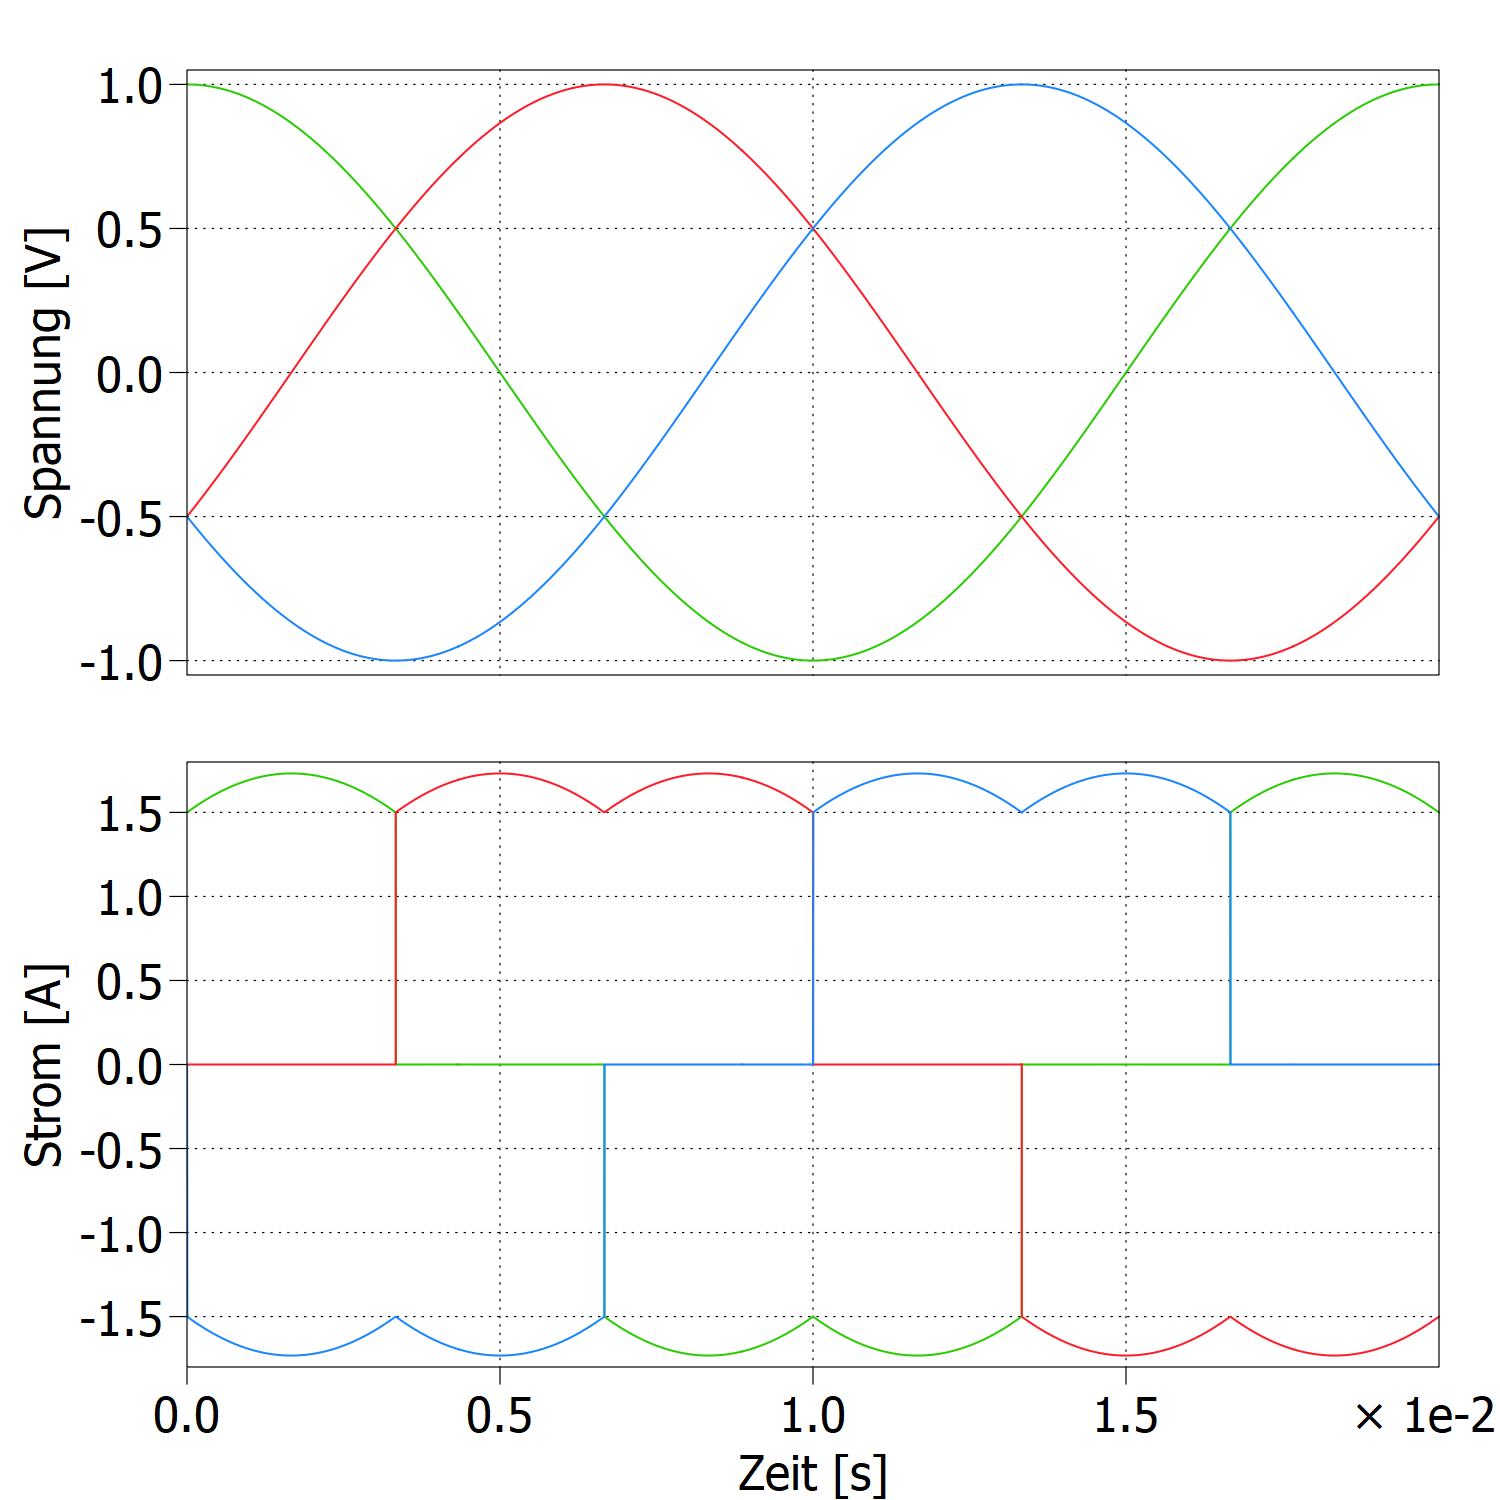
\includegraphics[width=0.7\linewidth]{content/Grafiken/B6-Diodengleichrichter-Eingangsverlauf}
			\caption{Strom und Spannungsverlauf am B6 Diodengleichrichter}
			\label{fig:B6DiodRect}
		\end{figure}
		
		Für Elektrolyseanlagen mit mehreren Megawatt Leistung müssen Zwangsweise Leistungshalbleiter parallelisiert werden, da bei Spannungen bis 1000 V die Ströme für einzelne Halbleiter zu hoch sind. Außerdem bietet die Parallelisierung durch Interleaving und Phasenverschiebung deutliche Vorteile für die Verzerrung und damit Filterung. Durch Thyristor basierte Schaltungen können große Leistungen effizient umgesetzt werden, jedoch führen diese zu deutlichen Verzerrungen des Stromverlaufs und schlechterem Leistungsfaktor. Daher benötigen diese passive oder aktive Filter, welche die Systemkosten erhöhen \cite{HydrogenElectronicTopologies}.
		Als Alternative dazu werden \gls{AFE} Gleichrichter eingesetzt diese bieten deutlich geringere Verzerrungen und völlige Freiheit bei der Regelung des Eingangsstroms. Daher können die Filter und Blindleistungskompensation in diesem Fall eingespart werden \cite{HydrogenElectronicTopologies}.
		
		\subsection{DC-DC Wandler} \label{sec:Buck}
		Der Hoch- und Tiefsetzsteller sind essenzielle Topologien und bestehen im wesentlichen aus zwei Halbleitern und einer Induktivität. In Abb. \ref{fig:buck} ist die Schaltung für einen Tiefsetzsteller zu sehen. Über das \gls{D} des Schalters kann die \gls{Ua} eingestellt werden, dabei sind die Parameter \gls{Ue}, Lastimpedanz sowie Wert der Induktivität relevant. Die Ausgangsspannung lässt sich im nicht lückendem Betrieb über den Zusammenhang $U_{out}=D\cdot U_{in} $ berechnen \cite{schmidtwalter}.\\
		\begin{figure}
			\centering
			\includegraphics[width=0.7\linewidth]{content/Grafiken/Buck}
			\caption[Tiefsetzsteller]{Tiefsetzsteller}
			\label{fig:buck}
		\end{figure}
		Die Speicherdrossel des Tiefsetzstellers kann über Formel \ref{eq:BuckL} ausgelegt werden, der gewünschte Stromrippel wird dazu beispielhaft auf maximal 30 Prozent des \gls{Ia} festgelegt \cite{schmidtwalter}.
		\begin{equation}
			\label{eq:BuckL}
			L=\dfrac{U_{emax}-U_{a}}{f\cdot 0,3 \cdot I_{a}}\cdot \dfrac{U_{a}}{U_{emax}}
		\end{equation}
		Wenn die Eingangsspannung durch einen, wie in Abb. \ref{fig:B6DiodRect} dargestellten, Dreiphasigen Diodengleichrichter implementiert ist, kann die Eingangsspannung mit $U_{LL} \cdot \sqrt{2}$ berechnet werden. Daraus folgt Formel \ref{eq:BuckLB6} bezogen auf die Phasenspannungen. \\
		\begin{equation}
			\label{eq:BuckLB6}
			L=\dfrac{U_{LL} \cdot \sqrt{2}-U_{a}}{f\cdot 0,3 \cdot I_{a}}\cdot \dfrac{U_{a}}{U_{LL} \cdot \sqrt{2}}
		\end{equation}
		Eine weitere Optimierungsmöglichkeit bietet das Interleaving, hierbei werden zwei Schaltungen parallel betrieben und die Regelung gekoppelt, dass Sie abwechselnd schalten. Dies ermöglicht es zum einen die Drosseln besser auslasten zu können und zum anderen den Rippel zu halbieren. 
		
		
		\subsection{Power Factor Correction (PFC)}
			Die \gls{PFC} ist eine nötige Maßnahme um den Blindleistungsanteil im Netz zu reduzieren und wird daher in aktuellen Geräten Standardmäßig implementiert. Ein Beispiel aus der Industrie bei dem bereits eine einfache Blindleistungskompensation durchgeführt wurde, war bei Leuchtmitteln mit Halogenröhren. Diese wurden zur Erzeugung der nötigen Spannung mit einem Transformator ausgestattet, welcher jedoch Blindleistung verursachte, dies konnte durch einfache Ergänzung eines Kondensators optimiert werden. \\
			In gängigen Gleichrichtersystemen werden getrennte Einheiten bestehend aus einer dreiphasigen PFC-Gleichrichterschaltung und einem Gleichspannungswandler (DC/DC-Buck-Wandler) eingesetzt, um die Anforderungen zu erfüllen. Die Regelung der beiden Wandlerstufen ist in der Regel entkoppelt, wobei der Gleichrichter sinusförmige Netzströme zieht und der nachfolgende DC/DC-Wandler die Spannung auf den erforderlichen Ausgang anpasst. Auf der Suche nach kompakten und leichten Systemen sind hohe Schaltfrequenzen notwendig, was jedoch zu erhöhten Schaltverlusten und verringerter Wandlereffizienz führen kann. Um dies zu adressieren, werden fortgeschrittene Modulationstechniken wie Einfügen der dritten harmonischen und Raumzeigermodulation möglich. Alternativ kann auch Diskontinuierliche Pulsweitenmodulation (DPWM) als Methode zur Reduzierung der Schaltverluste in dreiphasigen PFC-Gleichrichtern verwendet werden, um sinusförmige Eingangsströme und eine konstante Gleichspannung sicherzustellen. Im Gegensatz dazu müssen Einstufen-Wandlersysteme beide Anforderungen gleichzeitig erfüllen, während Zweistufen-Systeme trotz niederfrequenter Spannungsschwankungen im Zwischengleichspannungsnetz eine konstante Ausgangsspannung sicherstellen können.			
			
\section{IAF Rectifier }
Der \gls{IAF} Gleichrichter wurde erstmals vorgestellt in \cite{IAFfirst} im Jahr 1997, zur Verwendung in Photovoltaik Anwendungen. Dieser besteht für den Hauptleistungspfad aus einem Diodengleichrichter. Um sinusförmige Ströme in allen drei Phasen einzuprägen wird dieser durch ein Netzwerk aus bidirektional Sperrenden Leistungshalbleitern mit einer Induktivität und Halbbrücke ergänzt, dies wird als \gls{THI} Schaltung bezeichnet. Durch die Integration des Filters in den Leistungspfad, wird keine externe Blindleistungskompensation benötigt und die Filter können kleiner ausfallen. Aufgrund des ungesteuerten Diodengleichrichters wird jedoch eine anschließende Spannungsregelung durch einen Tiefsetzsteller benötigt \cite{ThesisSchrittwieserBuckTypePFC_2017}.\\
Das Netzwerk aus bidirektionalen Schaltern, auch als \gls{IVS} bezeichnet, ermöglicht das Schalten zwischen den einzelnen Phasen, in welche durch die Induktivität und Halbbrücke der gewünschte Sinusförmige Stromverlauf eingeprägt wird. Dazu schaltet die Halbbrücke hinter der Induktivität entweder zum positiven oder negativen Potential der \gls{Upn}. Der Diodengleichrichter bezieht immer nur aus zwei Phasen Strom, daher prägt die Schaltung, ohne Phasenverschiebung, nur in die jeweils dritte Phase Strom ein. Die Dioden und der \gls{IVS} schalten mit Netzfrequenz, um während der kommutierungsphase von 
\begin{figure}
	\centering
	\includegraphics[width=0.9\linewidth]{content/Grafiken/IAF}
	\caption[\gls{IAF} Gleichrichter Topologie]{\gls{IAF} Gleichrichter Topologie}
	\label{fig:iaf}
\end{figure}


\section{1/3 PWM PFC Rectifier}
\label{sec:GrundlagenB6}
Bei dieser Topologie handelt es sich um eine verbreitete B6-Topologie, die aus drei Halbbrücken besteht die jeweils an einer Phase angeschlossen sind. Durch ein adaptives Modulationsverfahren, unter Verwendung von Induktivitäten auf der Netzseite, wird eine Reduzierung der Schaltverluste und \gls{SDL} ermöglicht. Das Verfahren wurde ausführlich von Menzi, Bortis und Kolar beschrieben \cite{13PWMPFC}. Zur Regelung der Ausgangsspannung wird ein entkoppelter Tiefsetzsteller eingesetzt.\\



\begin{figure}
	\centering
	
\includegraphics[width=0.9\linewidth]{content/Grafiken/B6_Buck}
	\caption[1/3 PWM PFC Buck]{1/3 PWM PFC Buck}
	\label{fig:b6buck}
\end{figure}

Das besondere an der Regelung ist es, dass die Phase die aktuell keinen Strom führt, da Sie die niedrigste Spannung hat, durch \gls{PWM} Ansteuerung der zugehörigen Halbbrücke einen passenden Stromfluss erreicht. Die beiden anderen Halbbrücken werden jeweils wie ein Diodengleichrichter geschaltet. Dieses verfahren ist vom Prinzip her das gleiche, wie beim \gls{IAF} und kann daher zum Verständnis gemeinsam betrachtet werden, siehe Abb. \ref{fig:b6iafsectors}.
Im hervorgehobenen Abschnitt ist Phase b am niedrigsten und es ist zu sehen, in Bereich (f), dass nur eine Halbbrücke per \gls{PWM} angesteuert wird. In Bereich (e) wird der Tastgrad \gls{D} dargestellt, wobei der Wert 1 die dauerhafte Verbindung zum positiven und -1 die zum negativen Potential des Zwischenkreis \gls{Upn} darstellt \cite{13PWMPFC}.\\ 

\begin{figure}
	\centering
	\includegraphics[width=0.9\linewidth]{content/Grafiken/B6+IAF_Sectors.png}
	\caption[Sektorenaufteilung und Schaltverhalten von IAF und B6 1/3 \cite{13PWMPFC}]{}
	\label{fig:b6iafsectors}
\end{figure}

\section{Leistungshalbleiter}
Halbleiter sind prinzipiell alle Komponenten mit mindestens einem PN-Übergang, wenn diese größere Leistungen Schalten können, werden sie als Leistungshalbleiter bezeichnet. Dazu sind für die verwendete Topologie, neben der klassischen Diode, \gls{MOSFET}  relevant. Diese lösen in der Leistungselektronik aktuell den verbreiteteren IGBT oftmals ab aufgrund der günstiger gewordenen Silicium Carbide Variante \cite{SiCTrend}. Die Vorteile dieser neuen Technologie liegen in der Ermöglichung höherer Schaltfrequenzen, dies wiederum ermöglicht die Reduzierung der Energie welche in den Induktiven Komponenten gespeichert werden muss und spart somit Kosten.\\
Um die am besten geeigneten Halbleiter auszuwählen werden u.a. Simulationen der Schaltung verwendet, diese benötigen eine Nachbildung der Halbleiter. Um die Modelle der Leistungshalbleiter zu erstellen und ggf. vorhandene zu validieren, können Messungen mittels \gls{DPT} durchgeführt werden. Ein Beispiel der in \gls{PLECS} dargestellten Ausschaltverluste für einen Halbleiter können in Abb. \ref{fig:plecsff2thermalmodel} gefunden werden. Es ist zu sehen, dass die Punkte nur für den Betriebspunkt von 600 Volt zur Verfügung stehen, für andere Betriebsbereiche muss das Verhalten approximiert werden. Außerdem wird der \gls{RGV} nur für einen Begrenzten Bereich dargestellt und die \gls{VGSS} nur auf einen Wert beschränkt. Dies kann für die spätere Anwendung zu deutlichen Abweichungen führen.
\begin{figure}
	\centering
	\includegraphics[width=0.7\linewidth]{content/Grafiken/PLECS_FF2ThermalModel}
	\caption[Darstellung der Ausschaltverluste \cite{IFAGFF2}]{Darstellung der Ausschaltverluste \cite{IFAGFF2}}
	\label{fig:plecsff2thermalmodel}
\end{figure}

\section{Induktive Komponenten}
Als Induktive Komponenten werden in der Regel Spulen und Transformatoren betrachtet, diese dienen dazu Energie zu Speichern und zu Übertragen. Transformatoren bieten zusätzlich die Möglichkeit der galvanischen Entkopplung von Stromkreisen.\\ 
Zur Auslegung von Induktivitäten wird das Delta des Stroms in der Spule benötigt, der sogenannte Stromrippel. Dieser Strom wird meist auf 30 Prozent des Effektivstroms ausgelegt. Der Rippelstrom für Drehstromsysteme kann über Formel \ref{eq:DeltaI} bestimmt werden. Dabei ist die \gls{S} und \gls{Ull} die Spannung zwischen den Außenleitern.\\
\begin{equation}
	\label{eq:DeltaI}
	 \Delta I = 0,3 \cdot \dfrac{\sqrt{2} \cdot S}{2 \cdot \sqrt{3} \cdot U_{LL}}
\end{equation}
Außerdem kann über die gespeicherte Energie in der Drossel eine Aussage darüber getroffen werden, wie groß und damit indirekt wie viel kosten und Platzbedarf diese benötigt.

FORMELN MIT QUELLENNN!!!!!!



\section{Simulationssoftware}
Zur Bewertung und Betrachtung der Umsetzbarkeit, der Topologien ist es nötig diese in einer Umfassenden Simulation zu betrachten. Dies ermöglicht es die Funktionalität und den Einfluss der Parameter im direkten Zusammenspiel zu untersuchen. Insbesondere das Verhalten für Systemdienstleistungen, wie Phasenverschiebung und die dadurch beeinflusste Verteilung der Verlustleistungen sollen als Entscheidungsgrundlage dienen. 

	\subsection{PLECS}
	Die Software \gls{PLECS} aus dem Haus PLEXIM wird als Integration in MATLAB mit Simulink verwendet.  Diese ermöglicht die Modellierung von Schaltungen mit der Betrachtung des Thermischen Verhaltens durch elektrische Modelle der Verlustleistung. Dazu wird die Energie im Schaltvorgang sowie im durchgeschalteten Zustand in der Schaltung berücksichtigt. Dies ermöglicht es die Verlustleistung innerhalb der Halbleiter zur betrachten und damit den Aufwand für die Kühlung und eine Abschätzung der Schaltungseffizienz. Ein Beispiel der Funktionen kann in Abb. \ref{fig:plecsbuck} gesehen werden, die thermische Kette muss anhand von Datenblättern oder ähnlichem der Kühlkörper bekannt sein. Für die Halbleiter werden thermische Modelle benötigt, die ebenfalls aus Datenblättern erstellt oder vom Hersteller bereitgestellt werden können. Jedoch gibt es nicht für alle Halbleiter ausreichend Informationen und die reale Verlustleistung hängt von vielen Parametern ab. Daher wird es oftmals benötigt eigene Messungen durchzuführen, um die spätere Anwendung bestmöglich simulieren zu können.   \\
	
	\begin{figure}
		\centering
		\includegraphics[width=0.9\linewidth]{content/Grafiken/PLECS_Buck}
		\caption[Tiefsetzsteller mit Effizienzbestimmung]{Tiefsetzsteller mit Effizienzbestimmung}
		\label{fig:plecsbuck}
	\end{figure}
	
\chapter{Anforderungen}
\label{chap:Anforderungen}

\section {Stromnetz}
In Deutschland sind die Vorgaben für den Anschluss von Anlagen an das Stromnetz durch den \gls{VDE} definiert. Je nach Anschlussleistung wird eine unterschiedliche Netzspannungsklasse gewählt, welche geringfügig abweichende Anschlussrichtlinien besitzt. Aufgrund der Skalierbarkeit zu höheren Leistungsklassen und der erwartbar steigenden Anforderungen, wird sich für die Bestimmungen für Hochspannung entschieden. Diese hat die Bezeichnung VDE-AR-N 4120 "Technische Regeln für den Anschluss von Kundenanlagen an das Hochspannungsnetz und deren Betrieb (TAR Hochspannung)" \cite{VDEARN4120} . 

\subsection{Systemanforderungen}


\subsection{Überspannungsschutz}

\section{Elektrolyse}

\chapter{Simulation}

\section{Randbedingungen}

Die Regelung benötigt eine Erkennung des aktuellen Phasenwinkelabschnitts, diese ist implementiert nach \cite{InstituteofElectricalandElectronicsEngineers}.

\section{IAF}

\cite{IAF99}


\section{B6 1/3 PFC Buck}
\chapter{Simulation}
Die Simulationen sind vom Grundaufbau her wie folgt implementiert: Sie bestehen aus einem Konfigurationsskript, das die Parameter für das eigentliche Modell in den Matlab Workspace lädt und die Automatisierung der Simulationsläufe implementiert. Das Modell wird in Simulink über das PLECS Blockset aufgebaut und die Daten werden über eine Ausgabe als gebündelte Schnittstelle an Matlab zurückgegeben. Die Rückführung der Daten erfolgt einheitlich für die Simulationen in einer festgelegten Reihenfolge, siehe Abb. \ref{fig:plecsout}. Dies ermöglicht eine einheitliche Auswertung und Speicherung der Daten, zur Begrenzung der Datenmenge wird die Anzahl der Messpunkte auf die letzte Sinusperiode begrenzt. Die Schaltung und die zugehörige Steuerung befinden sich in jeweils eigenen PLECS-Systemen, für das Netz und den Elektrolyseur ist ein eigenes Subsystem vorgesehen, siehe Abbildung \ref{fig:plecssimulationsaufbau}.
\begin{figure} [H]
\centering
\includegraphics[width=1\linewidth]{content/Grafiken/PLECS_Simulationsaufbau}
\caption{Übersicht der PLECS Simulation}
\label{fig:plecssimulationsaufbau}
\end{figure}
Das Netz wird durch eine einfache Drehstromquelle dargestellt und kann in späteren Schritten durch Netzimpedanzen und Fehlerszenarien ergänzt werden. Der Elektrolyseur besteht der Einfachheit halber aus einem geeigneten Lastwiderstand, der im Betriebspunkt die gemäß Skript eingestellte Leistung aufnimmt. Zusätzlich werden Widerstände eingesetzt, um die Schaltung in \gls{PLECS} berechenbar zu machen, da sonst beim Einschaltvorgang durch Kapazitäten unendlich hohe Ströme entstehen würden. In der realen Anwendung treten diese als parasitäre Widerstände auf.
\begin{figure}
\centering
\includegraphics[width=1\linewidth]{content/Grafiken/Plecs_Out}
\caption{Zusammenfassung der Simulationsoutputs}
\label{fig:plecsout}
\end{figure}


\section{Randbedingungen}
Für den Gleichrichter werden grundlegende Parameter festgelegt, um die Auslegung für die Simulation durchführen zu können. Die Leistung von 200 kW wird als Grundlage festgelegt, da höhere Ströme aufgrund der Halbleitermodule und thermischen Belastung in einem Gerät Probleme bei der Umsetzung verursachen würden. Höhere Ströme würden die Stromtragfähigkeit gängiger Platinen übersteigen und damit die Kosten übermäßig steigern. Die Ausgangsspannung von maximal 680 V ergibt sich aufgrund der Spannungsfestigkeit der Halbleitermodule, welche 1200 V beträgt. Diese muss aufgrund von Spannungsspitzen bei Schaltvorgängen der Halbleiter weiter begrenzt werden. Aufgrund der Abschätzung der Kommutierungsinduktivität, die beim Schaltvorgang zu Überspannungen führt, welche die Lebensdauer der Halbleiter beeinträchtigen können, wird ein größerer Abstand zur Halbleiterspannung gewählt. Es wird sich für diese Spannungsklasse entschieden, da diese bereits etabliert und in breiter Masse verfügbar ist. Die Netzfrequenz sowie das Spannungsband wird anhand der Anforderungen für stationären Betrieb im deutschen Stromnetz definiert. Die Spannungsschwankung wird auf \pm 10 \% der Netznennspannung reduziert da kurzfristige Änderungen und entsprechende Kompensationen später betrachtet werden. Für die Simulation werden die in Tabelle \ref{tab:Betriebspara} aufgeführten Betriebsparameter verwendet. Die beiden Topologien werden verglichen, um die beste Lösung zu finden. Dabei wird der Einfluss der Systemdienstleistungen bei einem Phasenversatz von 0° und 30° der Eingangsströme berücksichtigt. Um die Eingangsströme bei Phasenverschiebung auszugleichen, wird die Ausgangsleistung um den Faktor cos(30°) reduziert. Die Kühlplattentemperatur von 80 °C wird aufgrund der Wahl einer Wasserkühlung für den Demonstrator gewählt.

\begin{table}
	\centering
	\caption{Auflistung der Simulationsbetriebsparameter}
	\begin{tabular}{c c}

		Ausgangsspannung \gls{Ua} & 680 V \\
		\hline
		Ausgangsleistung & 200 kW bei $\varphi = 0°$\\
		\hline
		Phasenverschiebung & 0 / 30 Grad \\
		\hline
		Kühlplattentemperatur & 80 °C \\
		\hline
		Schaltfrequenz & 20 kHz \\
		\hline
		Netzspannung \gls{Ull} & 617 \si{\volt} \\
		\hline
		Netzfrequenz &		50 Hz \\
		\hline
		Netzspannungsschwankung & 10 \% \\
	\end{tabular}
	\label{tab:Betriebspara}
\end{table}

Für die Auswertung wird der eingeschwungene Zustand des Systems betrachtet, dieser wird anhand des Temperaturverhaltens der Halbleiter kontrolliert. Dies erleichtert die Auslegung der Regler, die Parameter werden so gewählt, dass ein stabiler Zustand erreicht wird und keine Schwingungen auftreten. Außerdem wird für die Auswertung die letzte Periode der Simulation verwendet, da hier der thermische Vorgang eingeschwungen ist. Dieser Abschnitt wird für eine spätere Betrachtung gespeichert.

\section{Tiefsetzsteller}
Der Tiefsetzsteller kann entkoppelt vom Gleichrichter betrachtet werden, was für die Auslegung der Induktivität von Vorteil ist. Die Regelung kann ebenfalls entkoppelt erfolgen, sodass eine getrennte Stabilitätsbetrachtung und Optimierung möglich ist. 
	\subsection{Auslegung der Induktivität}
	Die Speicherdrossel wird nach der Formel \ref{eq:BuckL} ausgelegt, wobei die Netzspannung maximal $U_{LLmaxPeak}=1,1 \cdot 617\, \si{\V} \cdot \sqrt{2}=959,8\, \si{\V}$ und die Ausgangsspannung $U_{a,min}$ liegt bei mindestens 482 \si{\V}. Daraus ergeben sich die maximalen Parameter, die der Tiefsetzsteller realisieren muss. Es ergibt sich eine Induktivität von 134,16 \si{\micro \henry}, siehe Formel \ref{eq:BuckLwert}. Die gespeicherte Energie beträgt 7,78 Joule bei einem Ausgangsstrom von 295 A. 
	\begin{equation}
	\label{eq:BuckLwert}
	L_{T}= \dfrac{U_{LLmaxPeak}-U_{amin}}{f_{sw} \cdot \Delta I} \cdot D = \dfrac{959,8\,\si{\V} - 482\, \si{\V}}{20\, \si{\kilo \hertz}\cdot 0,3 \cdot 295\, \si{\ampere}} \cdot \dfrac{482\, \si{\V}}{959,8\, \si{\V}}= 134,16 \,\si{\micro \henry} 
	\end{equation}
	\begin{equation}
		E=\dfrac{1}{2} \cdot L_{T} \cdot I_{a}^{2} = \dfrac{1}{2} \cdot 134,16\, \si{\micro \henry}  \cdot 294\, \si{\ampere} = 7,78\, \si{\joule}
	\end{equation}
	\subsection{Regelung}
	Die Regelung kann mit den im Abschnitt \ref{sec:Buck} beschriebenen Eingangsspannungsverhältnissen ausgelegt werden. Der Tastgrad (Duty Cycle \gls{D}) ist das Verhältnis von Eingangsspannung zu Ausgangsspannung. Aufgrund der sechspulsigen Zwischenkreisspannung schwankt der Duty Cycle \gls{D} geringfügig, da eine feste Ausgangsspannung gewünscht ist, kann die Regelung mit einem PI-Regler realisiert werden.\\
	Der Tiefsetzsteller wird durch einen PI-Regler zur Fehlerkorrektur angesteuert, wobei der ideale Tastgrad aus der gewünschten Ausgangsspannung und der Zwischenkreisspannung \gls{Upn} als Vorsteuerung dient. Die gewünschte Ausgangsspannung \gls{Ua} wird durch den Sollstrom und den bekannten Lastwiderstand generiert. Der Tastgrad \gls{D} wird dann einem PWM-Generator zugeführt, der das Steuersignal mit der gewünschten Schaltfrequenz von 20 kHz erzeugt. Um die Schaltverluste und die Leitungsverluste beim Kommutieren in den Dioden zu berücksichtigen, wird eine Totzeit von 500 \si{\nano \second} eingestellt, siehe Abbildung. \ref{fig:iafbuckcontrol}.
	\begin{figure}[H]
		\centering
		\includegraphics[width=1\linewidth]{content/Grafiken/IAF_BuckControl}
		\caption{Regelung des Tiefsetzstellers des IAF}
		\label{fig:iafbuckcontrol}
	\end{figure}


\section{IAF}
	Der Schwerpunkt der Simulation liegt auf den Leistungshalbleitern, deren Anordnung in Abbildung \ref{fig:iafplecsmain}, \ref{fig:iafplecsbuck} und \ref{fig:iafplecsivs} zu entnehmen ist. Zur Bestimmung der Verlustleistung werden Modelle von Infineon verwendet, wobei die Dioden aus dem Modul FS100R12W2T7 \cite{FS100R12W2T7} verwendet werden und für den \gls{IVS} ein Modul mit 5 \si{\milli \ohm} \gls{SiC} \gls{MOSFET} ausgewählt wird. Die Halbbrücke an der Induktivität wird aus einem Modul mit 1,4 \si{\milli \ohm} aufgebaut \cite{FF4MR12W2M1H}. Alle Halbleiter haben eine Spannungsfestigkeit von 1200 V.
	\begin{figure}
		\centering
		\includegraphics[width=1\linewidth]{content/Grafiken/IAF_Plecs_main}
		\caption{Simulationsaufbau der Halbleiter des IAF}
		\label{fig:iafplecsmain}
	\end{figure}
	\begin{figure}
		\centering
		\includegraphics[width=1\linewidth]{content/Grafiken/IAF_Plecs_Buck}
		\caption{Simulationsaufbau der Halbleiter des Tiefsetzstellers vom IAF}
		\label{fig:iafplecsbuck}
	\end{figure}
	
	\begin{figure}
		\centering
		\includegraphics[width=0.7\linewidth]{content/Grafiken/IAF_Plecs_IVS}
		\caption{Simulationsaufbau der Halbleiter des IVS vom IAF}
		\label{fig:iafplecsivs}
	\end{figure}
	

	\subsection{Auslegung der Induktivitäten}
	Zur Auslegung der Induktivität wird vom Nennbetrieb ohne Phasenverschiebung ausgegangen. Dazu wird der $\hat{I}_{max}$ gebildet siehe Formel \ref{eq:Idachmax}, welcher durch Netzspannungsabfall um 10~\% maximal wird und somit 294,07 Ampere beträgt. Ohne Phasenverschiebung erreicht dieser bei 30 Grad der Sinuswelle sein Maximum, siehe Formel \ref{eq:IAF_I0}. Somit ergibt sich ein Spitzennennstrom $I_{IAF0°}$ von 147,04 Ampere.
	\begin{equation}
		\label{eq:Idachmax}
		\hat{I}_{max} = \dfrac{\sqrt{2} \cdot P   }{ \sqrt{3}  \cdot  U_{LLrms} \cdot 0,9} = \dfrac{\sqrt{2} \cdot 200\, \si{\kilo \watt}} { \sqrt{3} \cdot 617\, \si{V} \cdot 0,9} = 294,07\, \si{\A}
	\end{equation}
	
	\begin{equation}
		\label{eq:IAF_I0}
		I_{IAF0°}= sin(30°)\cdot \hat{I}_{max}=sin(30°)\cdot 294,07 \,A = 147,04\, \si{\A}
	\end{equation}
	
	Der Rippelstrom wird auf 30 \% des Nennstroms ausgelegt. Daher muss die Induktivität einen Wert von 272 \si{\micro \henry} haben, siehe Formel \ref{eq:Livs0}. Zur Bewertung der Induktiven Komponenten wird die gespeicherte Energie in der Drossel verwendet, diese berechnet sich nach Formel \ref{eq:EL_IVS0}
		
		\begin{equation}
			\label{eq:Livs0}
			L_{IVS0°}= \dfrac{U_{LLmaxPeak}}{4\cdot f_{sw} \cdot 0,3 \cdot I_{IAF0°}} = \dfrac{959,8\, V}{4 \cdot 20\, kHz \cdot 0,3 \cdot 147,04\, A}= 272\, \si{\micro \henry}
		\end{equation}
		
		\begin{equation}
			\label{eq:EL_IVS0}
			W_{L-IVS0°}=\dfrac{1}{2} \cdot L_{IVS} \cdot I_{IAF0°}^{2} = \dfrac{1}{2} \cdot 272\, \si{\micro \henry} \cdot (147,04\, \si{\A})^{2} =  2,94 \, \si{\joule}
		\end{equation}
		
		Bei der Betrachtung der Energie ist zu beachten, dass der Strom in der Drossel bei Blindleistung ansteigt und somit die Energie im quadratischen Verhältnis zunimmt. Bei Phasenverschiebung von 30 Grad ändert sich die Amplitude auf $sin(60°)$ und damit der Strom auf etwa 255 Ampere.
			
		
		
		\begin{equation}
			\label{eq:IAF_I30}
			I_{IAF30°}= sin(60°)\cdot \hat{I}_{max}=sin(60°)\cdot 294,07 \,A =254,68\, \si{\A}
		\end{equation}
		
		
		Die in der Drossel gespeicherte Energie, welche eine relevante Größe für die Bewertung darstellt, beträgt 8,82 Joule (siehe Formel \ref{eq:EL_IVS30}).
		
		\begin{equation}
			\label{eq:EL_IVS30}
			W_{L-IVS30}=\dfrac{1}{2} \cdot L_{IVS} \cdot I_{IAF30°}^{2} = \dfrac{1}{2}\cdot 272\, \si{\micro \henry} \cdot (254,68\, \si{\A})^{2} =  8,82 \, \si{\joule}
		\end{equation}
		
		
		
		Zusätzlich wird eingangsseitig eine Filterinduktivität $L_{IAF-N}$ mit dem Wert 1~\si{\micro \henry} eingesetzt, um das Verhalten des Netztrafos nachzubilden. Zur Bewertung der Induktiven Komponenten wird die gespeicherte Energie in der Drossel verwendet, dazu wird der Scheitelwert des Stroms $\hat{I}_{max}$ benötigt, siehe Formel \ref{eq:Idachmax}. Die Netzdrossel hat somit eine gespeicherte Energie von 0,1 Joule, siehe Formel \ref{eq:E_IAF_ACL}. Aufgrund der dreiphasigen Anwendung wird der Wert direkt mit dem Faktor 3 multipliziert.
			
			\begin{equation}
			\label{eq:E_IAF_ACL}
			W_{L-IAF-N}= 3\cdot \dfrac{1}{2} \cdot L_{IAF-N} \cdot (\hat{I}_{max})^2=\dfrac{3}{2} \cdot 1\, \si{\micro \henry} \cdot (294,07 \, \si{\ampere})^{2} = 0,13 \, \si{\joule}
		\end{equation}
	
	\subsection{Regelung}
		Die Regelung des Stroms des IVS wird anhand der Struktur von Soeiro et al. umgesetzt (vgl. Abb. \ref{fig:iafpapercontrol}) \cite{Soeiro.2013}.
		 \begin{figure}[H]
			\centering
			\includegraphics[width=0.8\linewidth]{content/Grafiken/IAF_Paper_Control}
			\caption{Struktur der Regelung des IAF \cite{Soeiro.2013}}
			\label{fig:iafpapercontrol}
		\end{figure}
		Die Umschaltung zwischen den Phasen erfolgt mithilfe einer vorhandenen PLL in PLECS zur Winkelbestimmung und anschließenden Sektorbestimmung. Die Sektorenzuweisung wird anhand des Phasenwinkels nach dem Schema aus Abbildung \ref{fig:b6iafsectors} umgesetzt. Die Auswahl der entsprechenden Schalter ist durch ein C-Skript implementiert (siehe Abbildung \ref{fig:plecsiafivscontrol}). 
		\begin{figure}[H]
			\centering
			\includegraphics[width=1\linewidth]{content/Grafiken/PlecsIAFivscontrol}
			\caption{PLECS Aufbau der \gls{IVS} Ansteuerung}
			\label{fig:plecsiafivscontrol}
		\end{figure}
			Der Strom in der Drossel wird durch den idealen Stromverlauf der mittleren Phase bestimmt. Der aktuelle Phasenwinkel der Spannung wird dazu durch die PLL erfasst und kann mit einer einstellbaren Phasenverschiebung verändert werden. Die Stromamplitude \gls{I^} wird über die Netzspannung und die gewünschte Ausgangsleistung bestimmt (siehe Formel \ref{eq:IdachTheory}). Der sinusförmige Strom wird durch die Amplitude und den entsprechenden Winkel mit jeweils 120° bzw. $\dfrac{2}{3}\pi$ Phasenversatz gebildet, siehe Abb. \ref{fig:plecsiafidealephasenstrome}. Die mittlere Phase wird über die Sektorenzuweisung ausgewählt, siehe Abbildung \ref{fig:plecsiafiy}.
			\begin{equation}
				\label{eq:IdachTheory}
				\hat{I} = \dfrac{\sqrt{2} \cdot P   }{ \sqrt{3} \cdot cos(\varphi) \cdot  U_{LLrms} } 
			\end{equation}
		\begin{figure}[H]
			\centering
			\includegraphics[width=1\linewidth]{content/Grafiken/PLECS_IAF_idealePhasenströme}
			\caption{Generierung der idealen Phasenströme}
			\label{fig:plecsiafidealephasenstrome}
		\end{figure}
		
		
		\begin{figure}[H]
			\centering
			\includegraphics[width=1\linewidth]{content/Grafiken/PlecsIAFiy}
			\caption{Bestimmung des Sollstroms der mittleren Phase}
			\label{fig:plecsiafiy}
		\end{figure}
		
	Der ideale Tastgrad K1 für den Strom in der Drossel wird über das Verhältnis der Spannungen durch den formelmäßigen Zusammenhang in Gleichung \ref{eq:K1} bestimmt. 
	\begin{equation}
		\label{eq:K1}
		K1 = \dfrac{U_{mid}- U_{low}}{U_{high} -U_{low}} 
	\end{equation}
Die Stromregelung erfolgt mithilfe eines diskreten PI-Reglerblocks aus der PLECS-Bibliothek. Die Signale zur Gate-Ansteuerung werden durch einen PWM-Generator erzeugt und anschließend durch eine Einschaltverzögerung zur Totzeit-Implementierung verzögert. Dieser Aufbau ist in Abbildung \ref{fig:plecsiafivsk1} dargestellt. 
		\begin{figure}
			\centering
			\includegraphics[width=1\linewidth]{content/Grafiken/PlecsIAFivsK1}
			\caption{Regelung des Stroms in der mittleren Phase}
			\label{fig:plecsiafivsk1}
		\end{figure}
		
		\subsection{Ergebnisse}
		Für die Auswertung werden die Simulationen für eine Dauer von bis zu zehn Sekunden durchgeführt, da zu diesem Zeitpunkt ein eingeschwungener Zustand erreicht ist. Wie in Abbildung \ref{fig:iaftemp0} zu erkennen ist, ist die Kühlplattentemperatur als Startpunkt auf 80~°C festgelegt. Die Temperatur der Dioden des Gleichrichters, welche den Hauptstrom führen, sind in grün dargestellt und ändern sich nur minimal aufgrund der Blindleistungsbereitstellung, siehe Abbildung \ref{fig:iaftemp30}. Die Temperatur beträgt knapp über 120~°C und liegt somit unterhalb der erlaubten Maximaltemperatur von 175~°C \cite{IFAGFF2}. Die Temperatur der T+/- Halbbrücke wird in Pink dargestellt und steigt bei Blindleistungsbereitstellung auf knapp 160~°C und bietet damit 15~°C Abstand zur zulässigen Maximaltemperatur.  Diese hohe Temperatur führt zwar nicht zu einem direkten Ausfall der Halbleiter, hat aber einen starken Einfluss auf die Lebensdauererwartung. Die Anzahl der Temperaturzyklen bei Temperaturen über 150~°C führt zu einem wahrscheinlichen Ausfall bei weniger als 10~000 Zyklen \cite{SicTemp}. Daher sollte eine Erhöhung der Chipfläche für die Halbbrücke am \gls{IVS} überlegt werden. Die Temperatur des Tiefsetzstellers wird in Rot dargestellt und sinkt aufgrund der reduzierten Ausgangsleistung bei Blindleistungsbereitstellung.  
		\begin{figure} 
			\centering
			\includegraphics[width=0.9\linewidth]{content/Grafiken/IAF_Temp_0Grad}
			
			
			\caption{Temperaturverhalten der Halbleiter des IAF ohne Phasenverschiebung}
			\label{fig:iaftemp0}
		\end{figure}
		
		\begin{figure} 
			\centering
			\includegraphics[width=0.9\linewidth]{content/Grafiken/IAF_Temp_30Grad}
			\caption{Temperaturverhalten der Halbleiter des IAF mit  Phasenverschiebung}
			\label{fig:iaftemp30}
		\end{figure}
		
		Die Simulationsergebnisse zeigen den erwarteten Strom- und Spannungsverlauf für die \gls{IVS} Induktivität mit einer Dreiecksform, siehe Abbildung. \ref{fig:iafacl}. Zusätzlich ist dem Eingangsstrom ein hochfrequenter Anteil überlagert, der durch die Schaltfrequenz des Tiefsetzstellers erklärt werden kann. Beim Schaltvorgang des \gls{IVS} treten starke Sprünge im Stromverlauf auf, da der Strom in der Induktivität zwischen den Phasen wechselt. Aufgrund der Eigenschaft der Spule, den gespeicherten Stromfluss aufrecht erhalten zu wollen, führt dies zu Sprüngen im Stromverlauf, da die Phasenströme zu diesem Zeitpunkt unterschiedlich sind und die Schaltvorgänge durch Totzeiten verzögert werden. Der Schaltpunkt liegt beim Maximum des Stromes in der Induktivität.\\
		In Abb. \ref{fig:iafacl30grad} wird dieses Problem durch den höheren Strom welcher in der Drossel des \gls{IVS} Pfades gespeichert und umgeschaltet werden muss noch verstärkt. Außerdem wird dadurch mehr Verlustleistung erzeugt. Dies ist auch in der Temperaturkurve in Abb. \ref{fig:iaftemp30} dargestellt. Es werden nur die höchsten Temperaturen dargestellt, dies sind die Eingangsdioden, beispielhaft an D1 in grün dargestellt sowie die \gls{MOSFET}s des T+ in pink (der Halbbrücke am \gls{IVS}), der \gls{IVS} in Gelb sowie des Tiefsetzstellers in rot. Ohne Blindleistung ist die Temperatur des IVS unter 90~°C und steigt durch den höheren Strom aufgrund der Phasenverschiebung um über 20~°C. Um den Sinusverlauf im Mittel besser erkennen zu können, ist in Abbildung \ref{fig:iafacl30grad} der Stromverlauf nach einer Tiefpassfilterung für die Schaltfrequenzanteile dargestellt. Dadurch ist die Phasenverschiebung besser ersichtlich, siehe Verlauf A Filter.
		\begin{figure}
			\centering
			\includegraphics[width=1\linewidth]{content/Grafiken/IAF_AC+L}
			\caption{Simulationsergebnisse des IAF ohne Phasenverschiebung, Eingangsspannung und Ströme, Strom in der IVS Induktivität }
			\label{fig:iafacl}
		\end{figure}
		\begin{figure}
			\centering
			\includegraphics[width=1\linewidth]{content/Grafiken/IAF_AC+L_30Grad}
			\caption{Simulationsergebnisse des IAF bei 30 Grad Phasenverschiebung, Eingangsspannung und Ströme, Strom in der IVS Induktivität }
			\label{fig:iafacl30grad}
		\end{figure}
		Die Topologie hat aufgrund der Anforderung an Blindleistungsbereitstellung einen Nachteil durch den IVS, da dieser sprunghafte Änderungen des Stromverlaufs verursacht. Diese starken Sprünge führen dazu, dass die THD des Stroms deutlich verschlechtert wird. Die THD liegt bereits ohne Phasenverschiebung bei etwa 15~\%, und mit Phasenverschiebung verdoppelt sich dieser Wert auf etwa 32 \%. Dies ist proportional zum vom \gls{IVS} geschalteten Drosselstrom, der sich ebenfalls etwa verdoppelt.  Somit kann der IAF den Anforderungen nur schwer gerecht werden, da weitere Filterstufen benötigt würden. Dies lässt sich auch gut anhand der Arbeit von Schrittwieser et al. sehen, welche den SWISS und \gls{IAF} mit 8~kW Leistung beschreibt. Bei ihrem Prototyp macht der EMI-Filter knapp 5\% mehr des Volumens aus als beim SWISS Rectifier \cite{IAF99}.
		
	

\section{B6-1/3-PWM PFC Buck}
Die in Kapitel \ref{sec:GrundlagenB6} beschriebene Schaltung wird mit insgesamt drei Halbbrückenmodulen der Firma Infineon realisiert, siehe Abb. \ref{fig:plecsb6}. Es handelt sich dabei um weit verbreitete 1200 \si{\volt} Module FF2MR12W3M1H, die einen nominellen Einschaltwiderstand von 2 \si{\milli \ohm} haben und Spitzenströme bis zu 800 \si{\ampere} schalten können \cite{IFAGFF2}.
\begin{figure}[H]
	\centering
	\includegraphics[width=1\linewidth]{content/Grafiken/PLECS_B6}
	\caption{PLECS Aufbau der B6 Leistungshalbleiter}
	\label{fig:plecsb6}
\end{figure}
 Um den gewünschten Ausgangsstrom bereitzustellen zu können sind für den Tiefsetzsteller zwei Halbbrückenmodule vorgesehen. Die Schaltung ist in Abbildung \ref{fig:plecsb6buck} zu finden. Es ist erkennbar, dass der Tiefsetzsteller durch den Kondensatoren C4 am Eingang des Tiefsetzstellers entkoppelt ist.
 \begin{figure}[H]
 	\centering
 	\includegraphics[width=0.9\linewidth]{content/Grafiken/PLECS_B6Buck}
 	\caption{PLECS Aufbau des Tiefsetzstellers der B6 Topologie}
 	\label{fig:plecsb6buck}
 \end{figure}
 

		\subsection{Auslegung der Netzinduktivität}
				Die Eingangsdrossel wird für den Normalbetrieb ausgelegt. Daher muss im Falle von Blindleistung die Wirkleistung reduziert werden. Wie bereits in Abschnitt \ref{sec:AnfStromnetz} erläutert, ist dies vom Netzbetreiber gestattet. Der Rippelstrom in der Drossel wird wie zuvor auf 30 \% der Grundschwingung ausgelegt, siehe Formel \ref{eq:Idachmax}. Der Rippelstrom beträgt somit 88,2 Ampere, siehe Formel \ref{eq:DeltaI_B6}.\\
			
			\begin{equation}
				\label{eq:DeltaI_B6}
				I_{\Delta max B6}= 0,3 \cdot \hat{I}_{max}= 0,3 \cdot 294,07\, \si{\A} = 88,2\, \si{\A}
			\end{equation}
			Die Induktivität kann nach der gleichen Beziehung wie für den \gls{IAF}-\gls{IVS} berechnet werden und beträgt 136 \si{\micro \henry}, siehe Formel \ref{eq:L_B6}.
			\begin{equation}
				\label{eq:L_B6}
				L_{B6}= \dfrac{U_{LLmaxPeak}}{4\cdot f{sw} \cdot I_{\Delta max B6}} = \dfrac{959,8\, \si{\volt}}{4 \cdot 20\, \si{\kilo \hertz} \cdot 88,2\, \si{\ampere}} =136\, \si{\micro \henry}
			\end{equation}
			Die in der Induktivität gespeicherte Energie wird ebenfalls durch den Zusammenhang zwischen Netzspannung und Ausgangsleistung definiert, erhöht sich jedoch nicht durch die Bereitstellung von Blindleistung. Die gespeicherte Energie pro Phase beträgt 5,88 Joule nach Formel \ref{eq:EL_B6} und muss aufgrund der dreiphasigen Ausführung mit dem Faktor drei multipliziert werden. Somit ergibt sich eine Gesamtenergie von 17,64 Joule für die Netzinduktivität der Topologie.
			
			\begin{equation}
			\label{eq:EL_B6}
			W_{LB6}= 3 \cdot \dfrac{1}{2} \cdot L_{B6} \cdot (\hat{I}_{max})^{2}= \dfrac{3}{2} \cdot 136 \,\si{\micro \henry} \cdot (294,07\, \si{\A})^{2} = 17,64 \, \si{\milli \joule}
			\end{equation}
		\subsection{Regelung}
			Die Regelung besteht aus einer vierstufigen Kaskadenstruktur, siehe Abbildung \ref{fig:b6-control-orig} (groß im Anhang \ref{fig:b6regelung}). Die erste Stufe ist die Ausgangsspannungsregelung, die aus Sollleistung und Netzspannung die gewünschte äquivalente Phasenimpedanz als Eingangsgröße für die Phasenstromregelung bildet. Die drei Regler für die Phasenströme bilden die zweite Stufe.\\
			In der dritten Stufe wird die Phase mit der mittleren Spannung ausgewählt und anhand der Phasenlage die Zwischenkreisspannung \gls{Upn} bestimmt. Die Zwischenkreisspannung ergibt sich als Sechspulsige-Gleichspannung und dient als Eingangsspannung für den Tiefsetzsteller. Die mittlere Phasenspannung wird als Referenz für den Tastgrad der entsprechenden Halbbrücke verwendet und prägt somit einen spannungsproportionalen Strom ein. Somit ist immer nur eine der drei Halbbrücken getaktet geschaltet, die anderen beiden sind wie bei einem Diodengleichrichter auf die jeweils positivste und negativste Spannung geschaltet. Die vierte Stufe ist der Tiefsetzsteller mit Reglern für den Eingangsstrom und die Ausgangsspannung.
				
			\begin{figure}
			\centering
			\includegraphics[width=1\linewidth]{content/Grafiken/B6-Control-orig}
			\caption{Regelung des \gls{B6PFC} \cite{13PWMPFC}}
			\label{fig:b6-control-orig}
			\end{figure}
		Die Ausgangsleistungsregelung in PLECS besteht aus einem PI-Regler (siehe Abbildung \ref{fig:plecsb6controlpout}), der die nominale Netzspannung mit der äquivalenten Netzimpedanz multipliziert und dann durch die aktuelle Netzspannung in die Soll-Phasenströme umwandelt. Um die Phasenverschiebung zu implementieren, wird der Sollstrom entsprechend des Phasenwinkels verzögert an die Regelung der B6-Ansteuerung weitergegeben.\\
				\begin{figure}
				\centering
				\includegraphics[width=0.9\linewidth]{content/Grafiken/PLECS_B6_ControlPout}
				\caption{PLECS Regelung der Ausgangsleistung als Sollgröße}
				\label{fig:plecsb6controlpout}
			\end{figure}
			Im nächsten Schritt wird die Regelung des Netzstroms durch einen weiteren PI-Regler implementiert. Die Erkennung der Phasenabschnitte wird mittels PLL und C-Skript umgesetzt. Siehe Abbildung \ref{fig:plecsb6controlrigrid}.  
				\begin{figure}
				\centering
				\includegraphics[width=0.9\linewidth]{content/Grafiken/PLECS_B6_ControlRiGrid}
				\caption{PLECS Regelung der Netzimpedanz und Phasenabschnittserkennung}
				\label{fig:plecsb6controlrigrid}
			\end{figure}
			Der Ausgang dieses Blocks dient einerseits mit der Sollgröße für die Zwischenkreisspannung $u\_pn*$ als Eingang für den Tiefsetzsteller und andererseits wird die Sollgröße der mittleren Spannung $u\_mid*$ als Eingang für die PWM-Erzeugung des \gls{B6PFC} Gleichrichters verwendet.\\
			Die Sollspannung der Mittenphase $U\_mid*$ dient als Eingangsgröße zur Erzeugung des PWM-Signals für die \gls{MOSFET}s. Dieses wird wiederum von einem PWM-Generator erzeugt und mit Hilfe eines C-Codes werden die Signale den entsprechenden Phasen im Sektor zugeordnet. Die Einschaltverzögerung dient der Totzeit-Implementierung, siehe Bild \ref{fig:plecsb6controlpwmmid}.\\
			\begin{figure}
				\centering
				\includegraphics[width=0.9\linewidth]{content/Grafiken/PLECS_B6_ControlPWMmid}
				\caption{PLECS PWM Erzeugung des B6 Gleichrichters mit \gls{PFC}}
				\label{fig:plecsb6controlpwmmid}
			\end{figure}
			Die Ansteuerung des Tiefsetzstellers, siehe Abb. \ref{fig:b6buckcontrol}, wird hier wie in der Vorlage (in Abbildung \ref{fig:b6-control-orig} dargestellt) durch zwei PI-Regler realisiert. Im Gegensatz zur Variante des \gls{IAF} wird hier die Zwischenkreisspannung \gls{Upn} berücksichtigt. Als zusätzlicher Schritt wird das PWM-Signal erzeugt und die Totzeit der Halbleiter durch Verzögerungsfunktionen umgesetzt.  
\begin{figure}
	\centering
	\includegraphics[width=1\linewidth]{content/Grafiken/B6_Buck_Control}
	\caption{Regelung des Tiefsetzstellers beim \gls{B6PFC}}
	\label{fig:b6buckcontrol}
\end{figure}		
\subsection{Ergebnisse}
			Es zeigt sich, dass der \gls{B6PFC} deutliche Nachteile bei den Induktivitäten und damit bei den Hardwarekosten hat. Die erforderliche dreiphasige Drossel führt dazu, dass der IAF in dieser Kategorie um mehr als 50\% besser abschneidet.
			Anders sieht es in den anderen Kategorien aus, wo weniger Kondensatoren benötigt werden. Die erforderliche B6-Schaltung enthält mehr \gls{MOSFET}, dafür aber keine Dioden. Bei der Verlustleistung zeigt sich der klare Vorteil der Topologie bei der Bereitstellung von \gls{SDL}, da sie fast keinen Einfluss auf die Verluste in den Halbleitern hat. Dies lässt sich anhand des Temperaturverhaltens in Abb. \ref{fig:b6temp030grad} bestätigen, durch die Reduzierung der Ausgangsleistung ist die Temperatur im \gls{MOSFET} FET7 des Tiefsetzsteller etwas niedriger, rosa dargestellt. Bei den Halbleitern der B6-Brücke ist praktisch kein Unterschied zu erkennen. Die Eingangsströme sind lediglich durch die Schaltimpulse leicht verrauscht und der Sinusverlauf folgt der Eingangsspannung wie gewünscht, siehe Abbildung \ref{fig:b6acdc0grad}.  Der Stromverlauf weist eine THD von nur etwa 5,8 \% auf.
			\begin{figure}
				\centering
				\includegraphics[width=1\linewidth]{content/Grafiken/B6_Temp_0&30Grad}
				\caption{Temperaturverhalten der Halbleiter des B6 mit und ohne Phasenverschiebung}
				\label{fig:b6temp030grad}
			\end{figure}
			\begin{figure}[H]
				\centering
				\includegraphics[width=1\linewidth]{content/Grafiken/B6_AC+DC_0Grad}
				\caption{Eingangs- und Ausgangsgrößen ohne Phasenverschiebung}
				\label{fig:b6acdc0grad}
			\end{figure}
			\pagebreak
			Mit einer Phasenverschiebung von 30 Grad sieht das Verhalten ähnlich aus, siehe Abbildung \ref{fig:b6acdc30grad}.  Der Stromverlauf weist eine etwas höhere THD von 7,1 \% auf, die jedoch durch geeignete Filter ausgeglichen werden kann.
			\begin{figure}
				\centering
				\includegraphics[width=1\linewidth]{content/Grafiken/B6_AC+DC_30Grad}
				\caption{Eingangs- und Ausgangsgrößen mit Phasenverschiebung}
				\label{fig:b6acdc30grad}
			\end{figure}
\section{Bewertung}
Die Ergebnisse der Gesamtbewertung sind in Tabelle \ref{tab:Auswertung} aufgeführt. Diese Tabelle enthält Informationen über die Hardware, insbesondere die Induktivitäten, sowie über die Kapazitäten, Halbleiter und Treiber. Zusätzlich werden die Ergebnisse der Simulation anhand der Verlustleistung der Halbleiter bewertet.  Zur Durchführung eines Vergleichs der Kategorien und einer Gesamtbewertung werden die Einzelkategorien zwischen null und eins normiert und mit einem Gewichtungsfaktor summiert. Die Kapazitäten haben nur einen vergleichsweise geringen Einfluss auf die Gesamtsystemkosten und werden daher nur mit fünf Prozent bewertet. Da die Drosseln einen größeren Einfluss haben, werden sie mit 50~\% gewichtet. Der Einfluss der Kondensatoren wird mit 5~\% berücksichtigt. Die restlichen 45~\% entfallen auf die Halbleiter in Form der Chipfläche (über den RDSON), die Anzahl der Treiber und die Verlustleistung. Die jeweiligen Punkte sind proportional zu erwartenden Systemkosten und Volumen. Daher stellt eine niedrigere Punktzahl eine bessere Bewertung dar. \\
\begin{table}
	\centering
	\caption{Auflistung der Simulationsergebnisse und Bewertung}
	\begin{tabular}{c|c|c|c|c}
		& Topologie & B6-Buck & \gls{IAF} & Gewichtung: \\
		\hline
		Induktivitäten& L1 Netzinduktivität \si{\micro \henry}& 136 & 1 &  \\
		\hline
		& Gespeicherte Energie J& 17,6 & 0,1 & \\
		\hline
		& L2 DC Induktivität \si{\micro \henry}& 136 & 136 &  \\
		\hline
		& Gespeicherte Energie J& 7,8 & 7,8 &  \\
		\hline
		& L3 IVS Induktivität \si{\micro \henry}& - & 302,2 &  \\
		\hline
		& Gespeicherte Energie J & - & 8,82 & \\
		\hline
		& \textbf{Induktivität normiert:} & \textbf{1}   & \textbf{0,66} & 50\% \\
		\hline
		Kapazitäten & C1 Netzkapazität \si{\micro \farad}& - & 50 &  \\
		\hline
		& C2 DC Ausgang mF& 1 & 1 &  \\
		\hline
		& C3 DC Zwischenkreis \si{\micro \farad}& 25 & 50 &  \\
		\hline
		& \textbf{Kapazität normiert:} & \textbf{0,26} &  \textbf{1} & 5\% \\
		\hline
		Halbleiter & SiC 4 \si{\milli \ohm} & 0 & 2 &  \\
		\hline
		& SiC 2 \si{\milli \ohm} & 10 & 4 &  \\
		\hline
		& SiC 5 \si{\milli \ohm} & 0 & 6 &  \\
		\hline
		& \textbf{MOSFET normiert:} & \textbf{1} &  \textbf{0,64} & 15\% \\
		\hline
		& Dioden & 0 & 6 &  \\
		\hline
		& \textbf{Dioden normiert} & \textbf{0} & \textbf{1} & 5\% \\
		\hline
		Treiber & Treiberanzahl & 8 & 7 &  \\
		\hline
		& \textbf{Treiber normiert:} & \textbf{1} & \textbf{0,88} & 5\% \\
		\hline
		Verluste in W & Schaltverluste 30 Grad & 567 & 503 &  \\
		\hline
		& Leitverluste 30 Grad & 254 & 1311 &  \\
		\hline
		& 30 Grad Gewichtung: & 75\% & 75\% &  \\
		\hline
		& Schaltverluste 0 Grad & 554 & 511 &  \\
		\hline
		& Leitverluste 0 Grad & 326 & 748 &  \\
		\hline
		& 0 Grad Gewichtung: & 25\% & 25\% &  \\
		\hline
		& \textbf{Verluste normiert:} &\textbf{0,5} & \textbf{1} & 20\% \\
		\hline
		\textbf{Gesamt} &  & \textbf{0,77} & \textbf{0,74} & \\
	\end{tabular}
	\label{tab:Auswertung}
\end{table}
\chapter{Auswertung}
In diesem Kapitel werden die Simulationsergebnisse dargestellt und zur Bewertung in Vergleichsparameter zusammengefasst. Für die Simulation werden die in Tabelle \ref{tab:Betriebspara} aufgeführten Betriebsparameter verwendet. Die beiden Topologien werden verglichen, um die beste Lösung zu finden, dabei wird um den Einfluss der Systemdienstleistungen zu berücksichtigen bei einem Phasenversatz von 0° und 30° der Eingangsströme betrachtet. Um die Eingangsströme bei Phasenverschiebung gleich zu halten wird die Ausgangsleistung reduziert um den Faktor $cos(30°)$ . Die Kühlplattentemperatur von 80 °C wird aufgrund der Wahl einer Wasserkühlung für den Demonstrator gewählt.

\begin{table}
	\centering
	\caption{Auflistung der Simulationsbetriebsparameter}
\begin{tabular}{|c|c|}
	\hline
	Netzspannung \gls{Ull} & 617 \si{\volt} \\
	\hline
	Ausgangsspannung \gls{Ua} & 680 V \\
	\hline
	Scheinleistung & 200 kW \\
	\hline
	Phasenverschiebung & 0 / 30 Grad \\
	\hline
	Kühlplattentemperatur & 80 °C \\
	\hline
	Schaltfrequenz & 20 kHz \\
	\hline
\end{tabular}

\label{tab:Betriebspara}
\end{table}


\section{IAF}
Für die Auswertung werden die Simulationen für eine Dauer von einer Sekunde durchgeführt, da zu diesem Zeitpunkt ein eingeschwungener Zustand erreicht ist. Das Temperaturverhalten der Halbleiter ist in Abbildung \ref{fig:iaftemp} dargestellt. Wie in Abbildung \ref{fig:iaftemp} dargestellt, ist die Kühlplattentemperatur als Startpunkt auf 80 °C festgelegt. Die Dioden des Gleichrichters, welche den Hauptstrom führen, sind in grün dargestellt und ändern sich nur minimal aufgrund der Blindleistungsbereitstellung. Die Temperatur beträgt knapp über 120 °C und liegt somit unterhalb der erlaubten Maximaltemperatur von 175 °C \cite{IFAGFF2}. Die Temperatur der T+/- Halbbrücke wird in Pink dargestellt und steigt bei Blindleistungsbereitstellung auf knapp 160 °C und bietet damit 15 °C Abstand zur zulässigen Maximaltemperatur. Die Temperatur des Tiefsetzstellers wird in Rot dargestellt und sinkt aufgrund der Reduzierten Ausgangsleistung bei Blindleistungsbereitstellung.  
\begin{figure}
	\centering
	\subfloat[][]{\includegraphics[width=1\linewidth]{content/Grafiken/IAF_Temp_0Grad}}
	\qquad
	\subfloat[][]{\includegraphics[width=1\linewidth]{content/Grafiken/IAF_Temp_30Grad}}
	\caption{Temperaturverhalten der Halbleiter des IAF ohne (a) und mit (b) Phasenverschiebung}
	\label{fig:iaftemp}
\end{figure}

Die Simulationsergebnisse zeigen den erwarteten Strom- und Spannungsverlauf für die Induktivität mit einer Dreiecksform, siehe Abbildung. \ref{fig:iafacl}. Zusätzlich ist dem Eingangsstrom ein hochfrequenter Anteil überlagert, der durch die Schaltfrequenz des Tiefsetzstellers erklärt werden kann. Außerdem treten beim Schaltvorgang des \gls{IVS} starke Sprünge im Stromverlauf auf, da der Strom in der Induktivität zwischen den Phasen schalten muss.\\
In Abb. \ref{fig:iafacl30grad} wird dieses Problem durch die starken Spannungsunterschiede zwischen den Phasen bei Phasenverschiebung noch verstärkt. Außerdem muss der \gls{IVS} mehr Strom führen und erzeugt dadurch mehr Verlustleistung. Dies ist auch an der Temperatur des in Abb. \ref{fig:iaftemp} dargestellten Kurven erkennbar. Es werden nur die höchsten Temperaturen dargestellt, dies sind die Eingangsdioden, beispielhaft an D1 in grün dargestellt sowie die \gls{MOSFET}s des T+ in pink (der Halbbrücke am \gls{IVS}), der \gls{IVS} in Gelb sowie des Tiefsetzstellers in rot. In (a) ist die Temperatur des IVS unter 90 °C und in (b) durch den höheren Strom aufgrund der Phasenverschiebung deutlich angestiegen. Um den Sinusverlauf im Mittel besser erkennen zu können, ist der Stromverlauf in Abbildung \ref{fig:iafacl30grad} zusätzlich nach einer Tiefpassfilterung dargestellt. Dadurch ist die Phasenverschiebung besser ersichtlich, siehe Verlauf A Filter.
\begin{figure}
	\centering
	\includegraphics[width=1\linewidth]{content/Grafiken/IAF_AC+L}
	\caption{Simulationsergebnisse des IAF ohne Phasenverschiebung, Eingangsspannung und Ströme, Strom in der IVS Induktivität }
	\label{fig:iafacl}
\end{figure}
\begin{figure}
	\centering
	\includegraphics[width=1\linewidth]{content/Grafiken/IAF_AC+L_30Grad}
	\caption{Simulationsergebnisse des IAF bei 30 Grad Phasenverschiebung, Eingangsspannung und Ströme, Strom in der IVS Induktivität }
	\label{fig:iafacl30grad}
\end{figure}
Die Topologie hat aufgrund der Anforderung an Blindleistungsbereitstellung einen Nachteil durch den IVS, da dieser sprunghafte Änderungen des Stromverlaufs verursacht. Diese starken Sprünge führen dazu, dass die THD des Stroms deutlich verschlechtert wird. Die THD liegt bereits ohne Phasenverschiebung bei etwa 15~\%, und mit Phasenverschiebung verdoppelt sich dieser Wert auf etwa 32 \%.  Somit kann der IAF den Anforderungen nur schwer gerecht werden, da weitere Filterstufen benötigt würden. Dies lässt sich auch gut anhand der Arbeit von Schrittwieser et al. sehen. Bei ihrem Prototyp macht der Filter knapp ein Viertel des Volumens aus \cite{IAF99}.

\section{B6-1/3-PWM PFC}
Es zeigt sich, dass der \gls{B6PFC} deutliche Nachteile bei den Induktivitäten und damit bei den Hardwarekosten hat. Die erforderliche dreiphasige Drossel führt dazu, dass der IAF in dieser Kategorie um mehr als 50\% besser abschneidet.
Anders sieht es in den anderen Kategorien aus, wo weniger Kondensatoren benötigt werden. Die erforderliche B6-Schaltung enthält mehr \gls{MOSFET}, dafür aber keine Dioden. Bei der Verlustleistung zeigt sich der klare Vorteil der Topologie bei der Bereitstellung von \gls{SDL}, da sie fast keinen Einfluss auf die Verluste in den Halbleitern hat. Dies lässt sich anhand des Temperaturverhaltens in Abb. \ref{fig:b6temp030grad} bestätigt werden, durch die Reduzierung der Ausgangsleistung ist die Temperatur im  \gls{MOSFET} FET7 des Tiefsetzsteller etwas niedriger, rosa dargestellt. Bei den Halbleitern der B6-Brücke ist praktisch kein Unterschied zu erkennen.
\begin{figure}
	\centering
	\includegraphics[width=1\linewidth]{content/Grafiken/B6_Temp_0&30Grad}
	\caption{Temperaturverhalten der Halbleiter des B6 mit und ohne Phasenverschiebung}
	\label{fig:b6temp030grad}
\end{figure}
Die Eingangsströme sind lediglich durch die Schaltimpulse leicht verrauscht und der Sinusverlauf folgt der Eingangsspannung wie gewünscht, siehe Abbildung \ref{fig:b6acdc0grad}.  Der Stromverlauf weist eine THD von nur etwa 5,8 \% auf. 

\begin{figure}
	\centering
	\includegraphics[width=1\linewidth]{content/Grafiken/B6_AC+DC_0Grad}
	\caption{Eingangs- und Ausgangsgrößen ohne Phasenverschiebung}
	\label{fig:b6acdc0grad}
\end{figure}
Mit einer Phasenverschiebung von 30 Grad sieht das Verhalten ähnlich aus, siehe Abbildung \ref{fig:b6acdc30grad}.  Der Stromverlauf weist eine etwas höhere THD von 7,1 \% auf, die jedoch durch geeignete Filter ausgeglichen werden kann.
\begin{figure}
	\centering
	\includegraphics[width=1\linewidth]{content/Grafiken/B6_AC+DC_30Grad}
	\caption{Eingangs- und Ausgangsgrößen mit Phasenverschiebung}
	\label{fig:b6acdc30grad}
\end{figure}

\section{Bewertung}
Die Ergebnisse der Gesamtbewertung sind in Tabelle \ref{tab:Auswertung} aufgeführt. Diese Tabelle enthält Informationen über die Hardware, insbesondere die Induktivitäten, sowie über die Kapazitäten, Halbleiter und Treiber. Zusätzlich werden die Ergebnisse der Simulation anhand der Verlustleistung der Halbleiter bewertet.  Zur Durchführung eines Vergleichs der Kategorien und einer Gesamtbewertung werden die Einzelkategorien zwischen null und eins normiert und mit einem Gewichtungsfaktor summiert. Da die Drosseln einen großen Einfluss haben, werden sie mit 50 Prozent gewichtet. Die Kapazitäten haben nur einen vergleichsweise geringen Einfluss auf die Gesamtsystemkosten und werden daher nur mit fünf Prozent bewertet. Die restlichen 45 Prozent entfallen auf die Halbleiter in Form der Chipfläche (über den RDSON), die Anzahl der Treiber und die Verlustleistung. Die jeweiligen Punkte sind proportional zu erwartenden Systemkosten und Volumen. Daher stellt eine niedrigere Punktzahl eine bessere Bewertung dar. \\
\begin{table}
	\centering
	\caption{Auflistung der Simulationsergebnisse und Bewertung}
	\begin{tabular}{|c|c|c|c|c|}
		\hline
		& Topologie & B6-Buck & \gls{IAF} & Gewichtung: \\
		\hline
		Induktivitäten& L1 Netzinduktivität \si{\micro \henry}& 136 & 1 &  \\
		\hline
		& Gespeicherte Energie J& 17,6 & 0,1 & \\
		\hline
		& L2 DC Induktivität \si{\micro \henry}& 136 & 136 &  \\
		\hline
		& Gespeicherte Energie J& 7,8 & 7,8 &  \\
		\hline
		& L3 IVS Induktivität \si{\micro \henry}& - & 302,2 &  \\
		\hline
		& Gespeicherte Energie J & - & 8,82 & \\
		\hline
		& \textbf{Induktivität normiert:} & \textbf{1}   & \textbf{0,66} & 50\% \\
		\hline
		Kapazitäten & C1 Netzkapazität \si{\micro \farad}& - & 50 &  \\
		\hline
		& C2 DC Ausgang mF& 1 & 1 &  \\
		\hline
		& C3 DC Zwischenkreis \si{\micro \farad}& 25 & 50 &  \\
		\hline
		& \textbf{Kapazität normiert:} & \textbf{0,26} &  \textbf{1} & 5\% \\
		\hline
		Halbleiter & SiC 4 \si{\milli \ohm} & 0 & 2 &  \\
		\hline
		& SiC 2 \si{\milli \ohm} & 10 & 4 &  \\
		\hline
		& SiC 5 \si{\milli \ohm} & 0 & 6 &  \\
		\hline
		& \textbf{MOSFET normiert:} & \textbf{1} &  \textbf{0,64} & 15\% \\
		\hline
		& Dioden & 0 & 6 &  \\
		\hline
		& \textbf{Dioden normiert} & \textbf{0} & \textbf{1} & 5\% \\
		\hline
		Treiber & Treiberanzahl & 8 & 7 &  \\
		\hline
		& \textbf{Treiber normiert:} & \textbf{1} & \textbf{0,88} & 5\% \\
		\hline
		Verluste W & Schaltverluste 30 Grad & 567 & 503 &  \\
		\hline
		& Leitverluste 30 Grad & 254 & 1311 &  \\
		\hline
		& 30 Grad Gewichtung: & 75\% & 75\% &  \\
		\hline
		& Schaltverluste 0 Grad & 554 & 511 &  \\
		\hline
		& Leitverluste 0 Grad & 326 & 748 &  \\
		\hline
		& 0 Grad Gewichtung: & 25\% & 25\% &  \\
		\hline
		& \textbf{Verluste normiert:} &\textbf{0,5} & \textbf{1} & 20\% \\
		\hline
		\textbf{Gesamt} &  & \textbf{0,77} & \textbf{0,74} & \\
		\hline
	\end{tabular}
	\label{tab:Auswertung}
\end{table}
\appendix					%Beginn des Anhangs, nummeriert in lateinischen Buchstaben
\backmatter					%Ende des Dokuments
%\printbibheading 
%\printbibliography[type=online,heading=subbibliography,title={Onlinequellen}]
\printbibliography
%\chapter*{Danksagung}
\begin{itemize}
	\item Vielen Dank an N. N.
\end{itemize}
%\cleardoublepage
%\listoftodos
\chapter{Inhalt der CD}

\begin{itemize}
	\item Master-Thesis
	\item Simulationsmodelle
		\subitem IAF.slx
		\subitem config.m für den IAF
		\subitem B6\_Buck.slx
		\subitem config.m für den B6 Buck
	
	\item Halbleitermodelle
\end{itemize}

\chapter{Anhang}

\setcounter{figure}{0}
\renewcommand{\thefigure}{A\arabic{figure}}

\setcounter{table}{0}
\renewcommand{\thetable}{A\arabic{table}}

\begin{figure}[H]
	\centering
	\includegraphics[width=0.65\linewidth]{content/Anhang/B6_Regelung}
	\caption{Regelungsstruktur des \gls{B6PFC} nach Menzi et Al. \cite{13PWMPFC}}
	\label{fig:b6regelung}
\end{figure}



\begin{table}
	\label{An:Entscheidungsmatrix}

\begin{tabular}{|c|c|c|c|c|c|}
	\hline
	Topologie & B6-1/3-PWM & Swiss & IAF & 6-Switch Buck & \% \\
	\hline
	L1 Netzinduktivität & 136 & 17,5 & 1 & 17,5 &\\
	\hline
	Gespeicherte Energie & 14,4 & 1,8 & 0,1 & 1,8 &\\
	\hline
	L2 DC Induktivität  & 136 & 136 & 136 & 136 &\\
	\hline
	Rippelstrom absolut & 88,5 & 88,5 & 88,5 & 88,5& \\
	\hline
	Gespeicherte Energie & 7,8 & 7,8 & 7,8 & 7,8 &\\
	\hline
	L3 IAF IVS Induktivität & - & - & 302,2 & - &\\
	\hline
	Gespeicherte Energie  & 0 & 0 & 2,6 & 0 &\\
	\hline
	Summe: & 22,2 & 9,6 & 10,6 & 9,6 &\\
	\hline
	\bfseries Induktivität normiert: & \bfseries 1 &\bfseries 0,43 &\bfseries 0,48 &\bfseries 0,43 & 50\\
	\hline
	C1 Netzkapazität & - & 50 & 50 & 50& \\
	\hline
	C2 am Elektrolyseur & 1 & 1 & 1 & 1 &\\
	\hline
	C3 DC Zwischenkreis & 25 & - & 50 & - &\\
	\hline
	\bfseries Kapazität normiert: &\bfseries 0,26 &\bfseries 0,5 &\bfseries 1 &\bfseries 0 &5\\
	\hline
	SiC 4mOhm & 0 & 0 & 2 & 0 &\\
	\hline
	SiC 2mOhm & 10 & 8 & 4 & 12 &\\
	\hline
	Vienna SiC 5mOhm & 0 & 6 & 6 & 0 &\\
	\hline
	\bfseries SiC normiert: &\bfseries 0,83 &\bfseries 0,87 &\bfseries 0,53 &\bfseries 1 &15\\
	\hline
	Vienna Diode & 0,0 & 6,0 & 6,0 & 0,0& \\
	\hline
	\bfseries Dioden normiert &\bfseries 0,0 & \bfseries1 &\bfseries 1 &\bfseries 0&5 \\
	\hline
	Treiberanzahl & 8 & 7 & 7 & 12 &\\
	\hline
	\bfseries Treiber normiert: &\bfseries 0,67 &\bfseries 0,58 &\bfseries 0,58 &\bfseries 1,00& 5\\
	\hline
	Schaltverluste 30 Grad & 567 & 215 & 503 & 303 &\\
	\hline
	Leitverluste 30 Grad & 254 & 1121 & 1311 & 543 &\\
	\hline
	Gewichtung 30 Grad & 75\% & 75\% & 75\% & 75\% &\\
	\hline
	Schaltverluste 0 Grad & 554 & 243 & 511 & 399& \\
	\hline
	Leitverluste 0 Grad & 326 & 781 & 748 & 722&\\
	\hline
	Gewichtung 0 Grad & 25\% & 25\% & 25\% & 25\%& \\
	\hline
	\bfseries Verluste normiert: &\bfseries 0,50 &\bfseries 0,75 &\bfseries 1,00 &\bfseries 0,55 &20\\
	\hline
	Gesamt &\bfseries 0,77 &\bfseries 0,6 &\bfseries 0,65 &\bfseries 0,55& \\
	\hline
\end{tabular}
\end{table}




		%Anhang hier einfügen
\end{document}